\documentclass[12pt, letterpaper]{article}

% =====================
% Paquetes
% =====================
\usepackage[utf8]{inputenc}
\usepackage[T1]{fontenc}
\usepackage[spanish]{babel}
\usepackage{lmodern}
\usepackage{setspace}
\usepackage[hyphens]{url}
\usepackage{amsmath}
\usepackage{geometry}
\usepackage{longtable}
\usepackage{booktabs}
\usepackage{tabularx}
\usepackage{fancyhdr}
\usepackage{array}
\usepackage{titlesec}
\usepackage{graphicx}
\usepackage{pdflscape} 
\usepackage{ragged2e}
\usepackage{multirow}
\usepackage{caption}
\usepackage{float}
% \usepackage[style=apa, backend=biber]{biblatex}
% \addbibresource{references.bib} % Archivo de bibliografía (no usado - bibliografía manual en references.tex)
\usepackage{xcolor}
\usepackage{hyphenat}
\usepackage{ragged2e} 
\usepackage{placeins}
\usepackage{csquotes}
\usepackage{pgfplotstable}
\geometry{margin=1in}
\setlength{\parindent}{1.27cm}
\setlength{\parskip}{1em}
\onehalfspacing

% Configuración títulos
\titleformat{\section}{\normalfont\bfseries\uppercase}{\thesection.}{1em}{}
\titleformat{\subsection}{\normalfont\bfseries}{\thesubsection.}{1em}{}
\renewcommand{\contentsname}{Índice}

% Encabezados y pies
\pagestyle{fancy}
\fancyhf{}
\fancyfoot[C]{\thepage}

% Estilo especial para páginas landscape
\fancypagestyle{landscapestyle}{
  \fancyhf{}
  \renewcommand{\headrulewidth}{0pt}
  \fancyfoot[R]{\smash{\raisebox{0.75\textheight}{\rotatebox{90}{\thepage}}}}
}

% Comando para rotar texto en tablas
\newcommand{\rot}[1]{\rotatebox{90}{\parbox{2cm}{\centering #1}}}

% =====================
% Documento
% =====================
% load hyperref as the last package to avoid redefinition/hook issues
\usepackage[hidelinks]{hyperref}
\let\cleardoublepage\clearpage

\begin{document}

% Portada
\begin{titlepage}
	\centering
	\includegraphics[width=5cm]{logo_universidad.png}\par
	\vspace{1cm}

	{\bfseries\LARGE Entrega final: Easy Transit\par}
	\vspace{2cm}
	{\large Autores: Jorge Luis Araque, Juan Camilo Velasquez, Juan David Tabares, Jhoan Esteban Corrales, Juan Esteban Cardona, Maicol Stiven Ruiz y Santiago Marin\par}
	{\large Docente: Alexánder Quintero\par}
	\vfill
	{\Large Facultad de Ingenierías, Universidad Tecnológica de Pereira \par}
	{\large Curso: Gerencia de Proyectos\par}
	{\large Pereira, Colombia \\ \today \par}
\end{titlepage}

\renewcommand{\contentsname}{Tabla de contenido}
% Índice
\tableofcontents
\newpage
\listoffigures
\newpage
\listoftables
\newpage

\section{Involucrados}

\begin{itemize}
    \item Usuarios
    \item Escuelas de conducción
    \item Centros de reconocimiento de conductores (CRC)
    \item Centros de enseñanza automovilística (CEA)
    \item RUNT (Registro Único Nacional de Tránsito)
    \item Ministerio de Transporte
    \item Secretaría de Tránsito de Pereira
    \item Entidades de salud (IPS)
    \item Agencias de seguros
    \item Proveedores de mensajería
    \item Gobernación de Risaralda y alcaldía local
    \item Entidades financieras
    \item Tramitadores
    \item AMCO (Área Metropolitana Centro Occidente)
    \item Asociación de Taxistas de Pereira
    \item ADITT (Asociación para el Desarrollo Integral del Transporte Terrestre Intermunicipal)
\end{itemize}
 

\section{Grupos de Involucrados}

\begin{itemize}
    \item \textbf{Particulares:}  
    Incluyen a las personas y actores individuales que interactúan directamente con el sistema de tránsito.  
        \begin{itemize}
            \item \textbf{Usuarios:} Personas que requieren tramitar su licencia. Son la población directamente beneficiada y quienes hacen uso de los servicios para poder conducir de forma legal.  
            \item \textbf{Tramitadores:} Personas que intermedian en procesos de tránsito para facilitar o agilizar la gestión documental de terceros.  
        \end{itemize}

    \item \textbf{Formación y certificación:}  
    Son las instituciones que garantizan la preparación y validación de las competencias necesarias para conducir.  
        \begin{itemize}
            \item \textbf{Escuelas de conducción:} Instituciones autorizadas para formar conductores en conocimientos teóricos y prácticos, asegurando que adquieran las competencias necesarias para manejar de manera segura.  
            \item \textbf{Centros de reconocimiento de conductores (CRC):} Entidades que realizan evaluaciones médicas, psicológicas y físicas para certificar que un aspirante está en condiciones de conducir.  
            \item \textbf{Centros de enseñanza automovilística (CEA):} Organizaciones que refuerzan la formación vial mediante cursos de actualización, reentrenamiento y programas complementarios.  
            \item \textbf{Entidades de salud (IPS):} Centros médicos habilitados para evaluar condiciones físicas, visuales y psicológicas de los aspirantes.  
        \end{itemize}

    \item \textbf{Estado:}  
    Entidades públicas responsables de regular, supervisar y garantizar el cumplimiento de las normas de tránsito.  
        \begin{itemize}
            \item \textbf{Ministerio de Transporte:} Entidad encargada de formular políticas, reglamentar y supervisar el sistema de transporte a nivel nacional.  
            \item \textbf{RUNT:} Base de datos nacional que centraliza información sobre conductores, vehículos y trámites, garantizando control y trazabilidad en el sistema de tránsito.  
            \item \textbf{Secretaría de Tránsito de Pereira:} Autoridad local responsable de trámites, sanciones, expedición de documentos y control de movilidad en la ciudad.  
            \item \textbf{Gobernación y alcaldía local:} Entidades territoriales que coordinan políticas de movilidad y tránsito en el departamento y municipio.  
        \end{itemize}

    \item \textbf{Empresas:}  
    Actores del sector privado que prestan servicios complementarios para el funcionamiento del sistema de tránsito.  
        \begin{itemize}
            \item \textbf{Agencias de seguros:} Compañías que ofrecen pólizas obligatorias y voluntarias relacionadas con el tránsito, como el SOAT.  
            \item \textbf{Entidades financieras:} Bancos y pasarelas de pago que permiten realizar las transacciones asociadas a trámites de tránsito.  
            \item \textbf{Proveedores de mensajería:} Empresas que apoyan en la entrega de documentos físicos como licencias y certificaciones.  
        \end{itemize}

    \item \textbf{Gremios:}  
    Asociaciones y colectivos que representan intereses de grupos de transporte y movilidad.  
        \begin{itemize}
            \item \textbf{AMCO:} Entidad pública que coordina proyectos de movilidad y transporte en Pereira, Dosquebradas y La Virginia.  
            \item \textbf{Asociación de Taxistas de Pereira:} Gremio que agrupa y representa a los conductores de taxi de la ciudad.  
            \item \textbf{ADITT:} Organización que representa a empresas y conductores del transporte intermunicipal.  
        \end{itemize}
\end{itemize}
  

\section{Mapa de involucrados (Mentefacto)}
\begin{figure}[H]
    \centering
    \includegraphics[width=1\linewidth]{involved/images/Gerencia_1.png}
    \caption{Mapa de Involucrados (Mentefacto)}
    \label{fig:placeholder}
    \vspace{0.2cm}
    \small Fuente: Elaboración propia.
\end{figure}

\section{Matriz de Problemas - Intereses Percibidos}
\begin{table}[H]
\centering
\begin{tabular}{|p{4cm}|p{5cm}|p{6cm}|}
\hline
\textbf{Involucrado} & \textbf{Interés} & \textbf{Problema} \\ \hline
Usuarios & Acceder a trámites de licencias de forma rápida y clara. & Trámites lentos y confusos. \\ \hline
Escuelas de conducción & Aumentar visibilidad y captar más estudiantes. & Baja difusión y exceso de competencia informal. \\ \hline
CRC & Más usuarios agendando exámenes médicos. & Desorden en citas y pérdida de usuarios. \\ \hline
CEA & Agilizar inscripción de aspirantes. & Procesos manuales que generan demoras. \\ \hline
RUNT & Garantizar trazabilidad y confiabilidad de la información. & Riesgo de falsificación y errores en registros. \\ \hline
Ministerio de Transporte & Mejorar digitalización y control. & Burocracia y lentitud en adopción digital. \\ \hline
Secretarías de Tránsito & Descongestionar oficinas. & Alta demanda presencial e ineficiencia. \\ \hline
IPS certificadoras & Optimizar atención de usuarios. & Retrasos y saturación de pacientes. \\ \hline
Agencias de seguros & Ofrecer pólizas asociadas a licencias. & Baja integración tecnológica. \\ \hline
Mensajería & Incrementar servicios de entrega. & Usuarios deben desplazarse a oficinas. \\ \hline
Gobernación y alcaldías & Modernización tecnológica. & Quejas por trámites presenciales lentos. \\ \hline
Entidades financieras & Facilitar pagos digitales. & Pagos presenciales con retrasos. \\ \hline
Tramitadores & Mantener ingresos. & Pérdida de demanda de sus servicios. \\ \hline
AMCO & Implementar procesos ágiles. & Persistencia de procesos lentos. \\ \hline
Asociación de Taxistas & Trámites ágiles y simples. & Trámites demorados y engorrosos. \\ \hline
ADITT & Trámites eficientes y accesibles. & Procesos ineficientes y desactualizados. \\ \hline
\end{tabular}
\caption{Matriz de problemas}

\end{table}


\section{Matriz de Expectativas - Fuerza}
\begin{table}[h]
\centering
\begin{tabular}{|p{4cm}|c|c|c|c|}
\hline
\textbf{Involucrado} & \textbf{Expectativa} & \textbf{Fuerza} & \textbf{Resultado} & \textbf{Rol} \\ \hline
Usuarios & 5 & 3 & 15 & Favorecedor \\ \hline
Escuelas de conducción & 3 & 3 & 9 & Favorecedor \\ \hline
CRC & 2 & 3 & 6 & Neutral \\ \hline
CEA & 2 & 3 & 6 & Neutral \\ \hline
RUNT & 4 & 5 & 20 & Favorecedor \\ \hline
Ministerio de Transporte & 4 & 5 & 20 & Favorecedor \\ \hline
Secretarías de Tránsito & 3 & 5 & 15 & Favorecedor \\ \hline
IPS certificadoras & 2 & 3 & 6 & Neutral \\ \hline
Agencias de seguros & 1 & 2 & 2 & Neutral \\ \hline
Mensajería & 1 & 2 & 2 & Neutral \\ \hline
Gobernación y alcaldías & 3 & 4 & 12 & Favorecedor \\ \hline
Entidades financieras & 2 & 3 & 6 & Neutral \\ \hline
Tramitadores informales & -5 & 1 & -5 & Neutral \\ \hline
AMCO & 4 & 3 & 12 & Favorecedor \\ \hline
Asociación de Taxistas & 4 & 3 & 12 & Favorecedor \\ \hline
ADITT & 4 & 3 & 12 & Favorecedor \\ \hline
\end{tabular}
\end{table}

\section{Análisis de Involucrados}
\justify
En primer lugar, los usuarios constituyen el grupo central, pues son los directamente
beneficiados con el acceso a trámites más rápidos, claros y económicos. Con una alta
expectativa y una fuerza considerable, su papel es claramente favorecedor, dado que
demandan soluciones que reduzcan costos y tiempos. Con la propuesta de licencia virtual
con código QR y validación biométrica, los usuarios se convierten en los principales
promotores del sistema, ya que podrán acceder a su documento de forma inmediata y
segura, sin depender de intermediarios.

Las escuelas de conducción, secretarías de tránsito, el RUNT, el Ministerio de
Transporte y las autoridades locales se ubican también como actores favorecedores. Estos
buscan mejorar la visibilidad de sus servicios, garantizar trazabilidad de la información,
digitalizar procesos y descongestionar las oficinas. La incorporación de un sistema
centralizado permitirá que el RUNT valide automáticamente la autenticidad de los datos,
que los CRC integren en línea los resultados de exámenes médicos y que las academias de
conducción registren el avance de los estudiantes, lo que fortalece la transparencia y control
institucional.

Por otra parte, entidades como los CRC, CEA, IPS certificadoras, agencias de
seguros, proveedores de mensajería y entidades financieras presentan un rol más neutral. Si
bien tienen intereses particulares en agilizar procesos o ampliar sus servicios, su influencia
es limitada y dependen de las decisiones de los actores principales para mejorar su
integración. En el nuevo esquema digital, estos actores deberán adaptarse a plataformas
automatizadas, lo que puede representar un reto tecnológico pero también una oportunidad
de modernización.

En cuanto a los gremios del transporte como AMCO, la Asociación de Taxistas de Pereira y la ADITT, muestran un papel favorecedor al representar colectivos que buscan
mayor organización, seguridad y eficiencia en la movilidad. Con la licencia digital, estos
gremios se benefician de un control más estricto de la legalidad de los conductores y la
reducción de fraudes en la expedición de documentos.

Finalmente, se identifican los tramitadores informales como un grupo detractor.
Estos actores ven amenazada su labor debido a la digitalización y simplificación de
trámites, pues el sistema reduce la necesidad de intermediación. Aunque su fuerza es
limitada, representan un riesgo potencial en la medida en que pueden generar resistencia o
prácticas indebidas.

En conclusión, la mayoría de los grupos de interés se alinean como favorecedores, lo
cual indica una alta probabilidad de éxito en la implementación del aplicativo tramite de licencia
virtual, siempre que se logre articular la participación de los diferentes niveles de gobierno,
instituciones educativas, gremios y usuarios finales. Los actores neutrales pueden
convertirse en aliados estratégicos si se integran adecuadamente, mientras que los
detractores deberán gestionarse con estrategias que mitiguen su resistencia. El uso de
tecnologías como el QR dinámico, la biometría y la centralización en el RUNT fortalece la
confianza del sistema y marca una transición hacia la modernización total de los trámites
de tránsito en Pereira.


\section{Arbol de Problemas}

\begin{figure}[H]
    \centering
    \includegraphics[width=0.9\linewidth]{trees/images/arbol_problemas.png}
    \caption{Arbol de Problemas.}
    \label{fig:placeholder}
    \vspace{0.2cm}
    \small Fuente: Elaboración propia.
\end{figure}

\subsection{Fundamentos del Árbol de Problemas}
\begin{itemize}

    \item \textbf{Poca integración locativa} \\
    En Pereira, la falta de articulación entre las oficinas de tránsito y la infraestructura urbana ha generado congestión y demoras en la atención. El crecimiento del parque automotor (43,4\% en 7 años) ha sobrepasado la capacidad física de los puntos de atención, lo que contribuye al caos vial y a la saturación de servicios.  
    \textbf{(El Pereirano, 2023)}

    \item \textbf{Poca productividad de los funcionarios} \\
    Los trámites para obtener licencias de conducción en Pereira pueden tardar entre uno y dos meses, incluso para procesos simples como la recategorización. Aunque existen plataformas como el RUNT, el proceso sigue siendo largo y requiere múltiples pasos presenciales, lo que refleja una burocracia persistente.  
    \textbf{(PaseDeMoto, 2025)}

    \item \textbf{Falta de personal de apoyo} \\
    El Instituto de Movilidad de Pereira enfrenta un déficit de al menos 120 agentes de tránsito, lo que limita la capacidad operativa para atender trámites y controlar el tráfico. Esta escasez de personal afecta directamente la eficiencia de los servicios y la seguridad vial.  
    \textbf{(RCN Radio, 2023; El Pereirano, 2023)}

    \item \textbf{Poca infraestructura tecnológica} \\
    Aunque el Instituto de Movilidad de Pereira ha invertido más de \$3.650 millones en modernización, los sistemas siguen mostrando rezagos que dificultan la eficiencia de los trámites.  
    \textbf{(El Pereirano, 2023)}

    \item \textbf{Procedimientos manuales} \\
    A pesar de los avances digitales, muchos trámites para licencias de tránsito en Risaralda aún dependen de procesos manuales, como entrega física de documentos, revisión operativa y archivo en libros. Esto ralentiza el flujo de atención y aumenta el margen de error.  
    \textbf{(PaseDeMoto, 2025)}

    \item \textbf{Problemática principal: Trámites para licenciaslentos y tediosos} \\
    En Pereira y el Eje Cafetero, la gestión de licencias de conducción presenta demoras constantes y procesos engorrosos. Se han registrado largas filas desde la madrugada en el Instituto de Movilidad para renovar el pase, reflejando la limitada capacidad operativa. A esto se suman las frecuentes caídas del RUNT, que en 2024 paralizaron trámites como expedición de licencias, renovaciones y cursos pedagógicos.  
    \textbf{(Concejo de Pereira, 2023; RCN Radio, 2024)}

    \item \textbf{Aumento de los reprocesos para los usuarios} \\
    Las fallas en el RUNT y la falta de interoperabilidad entre entidades generan reprocesos continuos. Cuando la plataforma entra en mantenimiento o falla, los usuarios deben reagendar servicios, volver a presentar documentos o repetir exámenes médicos, lo cual aumenta los costos emocionales y económicos.  
    \textbf{(Infobae, 2024)}

    \item \textbf{Pérdida productiva para los ciudadanos} \\
    El tiempo invertido en gestiones burocráticas reduce la productividad laboral. En promedio, una empresa en Colombia destina 2.620 horas al año a trámites administrativos, equivalente a un empleado de tiempo completo. En regiones como Risaralda, con abundantes trabajadores independientes y microempresarios, esta carga limita el tiempo dedicado a actividades productivas.  
    \textbf{(La República, 2025)}

    \item \textbf{Baja del PIB local} \\
    La acumulación de problemas burocráticos impacta negativamente el crecimiento económico. Colombia ha perdido posiciones en índices de competitividad internacional. En Risaralda, donde el transporte es clave para la economía, estos obstáculos reducen el impulso productivo.  
    \textbf{(La República, 2025)}

    \item \textbf{Aumento de costos para el Estado} \\
    La ineficiencia burocrática incrementa el gasto público. La necesidad de contratar personal eventual o mantener sistemas anticuados genera costos adicionales no previstos, reduciendo recursos disponibles para inversión en infraestructura o modernización tecnológica.  
    \textbf{(La República, 2025)}

    \item \textbf{Disminución del desempeño de inversión para el desarrollo} \\
    Los retrasos en la emisión de licencias afectan proyectos de infraestructura y movilidad. Grandes obras han quedado entrampadas en trámites administrativos, lo que conlleva sobrecostos, retrasos y menor confianza en las instituciones.  
    \textbf{(Valora Analitik, 2025)}
\end{itemize}

\section{Arbol de Soluciones}

\begin{figure}[H]
    \centering
    \includegraphics[width=1\linewidth]{trees/images/Arbol_Soluciones.png}
    \caption{Arbol de Soluciones.}
    \label{fig:placeholder}
     \vspace{0.2cm}
    \small Fuente: Elaboración propia.
\end{figure}

\section{Bibliografía}
\begin{itemize}
    \item El Pereirano. (2023). \textit{Problemas de movilidad y seguridad afectan a Pereira y Dosquebradas}. Recuperado de: \url{https://elpereirano.com/2023/05/06/problemas-de-movilidad-y-seguridad-afectan-a-pereira-y-dosquebradas}

    \item PaseDeMoto. (2025). \textit{Licencia de Conducción Pereira – Requisitos y Trámite}. Recuperado de: \url{https://pasedemoto.com/licencias-de-conduccion/pereira}

    \item RCN Radio. (2023). \textit{En Pereira hacen falta al menos 130 agentes de tránsito}. Recuperado de: \url{https://www.rcnradio.com/colombia/eje-cafetero/en-pereira-hacen-falta-al-menos-130-agentes-de-transito}

    \item El Pereirano. (2023). \textit{Déficit de 120 agentes de tránsito en Pereira}. Recuperado de: \url{https://elpereirano.com/2023/02/24/deficit-de-120-agentes-de-transito-en-pereira}

    \item Concejo de Pereira. (2023). \textit{Más agilidad en la renovación de licencias de conducción piden los concejales de Pereira}. Recuperado de: \url{https://www.concejopereira.gov.co/es/mas-agilidad-en-la-renovacion-de-licencias-de-conduccion-piden-los-concejales-de-pereira-EV2305}

    \item RCN Radio. (2024). \textit{Caídas del RUNT paralizan trámites en Pereira}. Recuperado de: \url{https://www.noticiasrcn.com/colombia/caidas-del-runt-paralizan-tramites-en-pereira-2024}

    \item Infobae. (2024). \textit{Pico y placa solidario, cursos pedagógicos y trámites en ventanilla única no podrán realizarse este lunes por cierre de la plataforma RUNT}. Recuperado de: \url{https://www.infobae.com/colombia/2024/06/24/pico-y-placa-solidario-cursos-pedagogicos-y-tramites-en-ventanilla-unica-no-podran-realizarse-este-lunes-por-cierre-de-la-plataforma-runt}

    \item La República. (2025). \textit{Una empresa en Colombia debe destinar 2.620 horas al año en trámites administrativos}. Recuperado de: \url{https://www.larepublica.co/economia/una-empresa-en-colombia-debe-destinar-2-620-horas-al-ano-en-tramites-administrativos-4210833}

    \item Valora Analitik. (2025). \textit{Los dos megaproyectos clave para Bogotá que aún no arrancan por trámites administrativos}. Recuperado de: \url{https://www.valoraanalitik.com/primicia-los-dos-megaproyectos-clave-para-bogota-que-se-adjudicaron-en-2022-y-no-han-arrancado-estas-son-las-razones}

    \item Corficolombiana. (2025). \textit{Informe sobre impacto económico de la tramitología en Colombia}.
\end{itemize}


\section{Matriz de Componentes, actividades, responsables y costos.}

\renewcommand{\arraystretch}{1.2} % Espaciado entre filas
\setlength{\tabcolsep}{5pt}       % Espaciado entre columnas

\begin{longtable}{|p{3.5cm}|p{6.5cm}|p{4.5cm}|}
	\caption{Matriz de Componentes, actividades, responsables y costos.}\label{tab:matriz}               \\
	\hline
	\textbf{Componente}                                      & \textbf{Actividad} & \textbf{Responsable} \\ \hline
	\endfirsthead
	\hline
	\textbf{Componente}                                      & \textbf{Actividad} & \textbf{Responsable} \\ \hline
	\endhead
	\hline
	\multicolumn{3}{r}{\textit{Continúa en la siguiente página}}                                         \\ \hline
	\endfoot
	\hline
	\multicolumn{3}{c}{\textit{Fuente: Elaboración propia.}}                                             \\ \hline
	\endlastfoot

	Procedimientos \newline automáticos                      &
	- Identificación de procesos \newline
	- Diseño de flujos automatizados \newline
	- Desarrollo de software  \newline
	- Pruebas y capacitación                                 &
	Ing. Sistemas \newline Grupo de Desarrollo \newline Jefes de Área                                    \\ \hline

	Alta integración  \newline locativa                      &
	- Diagnóstico de espacios físicos \newline
	- Reestructuración de áreas de \newline trabajo \newline
	- Implementación de mobiliario \newline ergonómico y tecnológico \newline
	- Adecuaciones eléctricas y de red                       &
	Área de Infraestructura \newline Arquitecto \newline Proveedores externos                            \\ \hline

	Alta productividad de los funcionarios                   &
	- Capacitación en uso de \newline herramientas digitales \newline
	- Implementación de programas de bienestar \newline
	- Evaluaciones periódicas                                &
	Talento Humano \newline Supervisores directos                                                        \\ \hline

	Suficiente personal de apoyo                             &
	- Reclutamiento de personal \newline administrativo y técnico \newline
	- Capacitación inicial \newline
	- Definición de roles y turnos \newline
	- Evaluación de desempeño del \newline personal de apoyo &
	Talento Humano \newline Coordinadores de Área                                                        \\ \hline

	Aumento de la infraestructura tecnológica                &
	- Compra de servidores y equipos \newline
	- Modernización del centro de datos \newline
	- Migración a la nube \newline
	- Implementación de ciberseguridad                       &
	Proveedor tecnológico \newline Área de TI \newline Jefes de Área                                     \\ \hline
\end{longtable}

\section{Análisis de alternativas}

\subsection{Alta integridad locativa}
Para la cual se desarrollarán las actividades de diagnóstico de espacios físicos, reestructuración de áreas de trabajo, implementación de mobiliario ergonómico y tecnológico, y adecuaciones eléctricas y de red. En este orden de ideas, para la elaboración de las tareas antes mencionadas, se encargará el área de infraestructura, un arquitecto y proveedores externos respectivamente.

\subsection{Procedimientos automáticos}
Este componente tendrá en cuenta las labores de identificación de procesos, diseño de flujos automatizados, implementación de software, y pruebas y capacitación. Para ello será necesario designar a un ingeniero de sistemas, un grupo de desarrolladores y jefes de área.

\subsection{Alta productividad de los funcionarios}
Se requiere de la capacitación en uso de herramientas digitales, la implementación de programas de bienestar y evaluaciones periódicas, que estarán a cargo del talento humano y los supervisores directos.

\subsection{Suficiente personal de apoyo}
Este componente requerirá reclutamiento de personal administrativo y técnico, capacitación inicial, definición de roles y turnos, y evaluación de desempeño del personal de apoyo. De estas labores se harán cargo el personal de talento humano y los coordinadores de área.

\subsection{Aumento de la infraestructura tecnológica}
Tendrá como labores fundamentales la compra de servidores y equipos, modernización del centro de datos, migración a la nube y la implementación de ciberseguridad, que estarán a cargo de un proveedor tecnológico, área de TI y jefes de área.


\section{Estructura analítica del proyecto (EAP)}

\begin{figure}[H]
	\centering
	\includegraphics[width=0.3\linewidth]{alternatives/images/Estructura analítica.png}
	\caption{Estructura analítica del proyecto (EAP).}
	\label{fig:eap}
	\vspace{0.2cm}
	\small Fuente: Elaboración propia.
\end{figure}

\section{Descripción del proyecto}

\subsection{Objetivos}

\subsubsection{Objetivo General}
Gestionar un sistema de trámites para licencias de conducción
ágil, eficiente y automatizado, que mejore la experiencia del
ciudadano.

\subsubsection{Objetivos Específicos}
\begin{itemize}
	\item Realizar el levantamiento y análisis de los requerimientos del sistema, identificando las necesidades del usuario y los requerimientos funcionales y no funcionales del proyecto.
	\item Diseñar la arquitectura y los componentes del sistema, definiendo los módulos, la estructura de datos y la interfaz de usuario.
	\item Desarrollar el código fuente del sistema siguiendo buenas prácticas de programación y asegurando la coherencia con el diseño propuesto.
	\item Efectuar pruebas de validación y verificación para evaluar la funcionalidad, eficiencia y confiabilidad del sistema.
	\item Elaborar la documentación técnica y de usuario que describa el funcionamiento, instalación y mantenimiento del sistema.
\end{itemize}

\subsection{Alcance}
Se propone implantar, en modalidad piloto y en una sede de la Secretaría de Tránsito de Pereira, una solución informática acotada para la etapa final del trámite de expedición de licencias de conducción a solicitantes por primera vez. El sistema estará compuesto por varios módulos funcionales que trabajarán de forma integrada para garantizar una atención ordenada, segura y trazable en las sedes de la Secretaría de Tránsito. A continuación, se describen los módulos principales que conformarán el sistema:

\subsubsection*{Módulo de gestión de llegada y turnos}
Este módulo atenderá el registro de la llegada de los ciudadanos y la administración de las colas de atención. Sus funciones
principales son:
\begin{itemize}
	\item Registrar la llegada del solicitante y asociarla al expediente correspondiente.
	\item Generar y asignar turnos de atención con estimación de tiempo.
	\item Mostrar la cola de atención para los funcionarios y permitir la llamada ordenada de turnos.
	\item Registrar horarios de inicio y término de la atención para efectos de control y reporte.
\end{itemize}

\subsubsection*{Módulo de verificación documental}
Este módulo permitirá la revisión guiada de los documentos exigidos antes de proceder con la entrega de la licencia. Sus funciones
principales son:
\begin{itemize}
	\item Presentar la lista de documentos mínimos requeridos por tipo de trámite.
	\item Registrar la constatación de cada documento y las observaciones del funcionario.
	\item Bloquear la emisión cuando falte un requisito crítico y generar las opciones de gestión correspondientes.
	\item Permitir la firma del funcionario responsable sobre la verificación realizada.
\end{itemize}

\subsubsection*{Módulo de conciliación de pagos}
Este módulo gestionará la verificación del pago del trámite y la emisión del recibo correspondiente. Sus funciones principales son:
\begin{itemize}
	\item Consultar el estado del pago asociado al expediente.
	\item Registrar la referencia de pago y generar el comprobante oficial.
	\item Gestionar la conciliación manual cuando sea necesario y registrar el resultado de la conciliación.
	\item Bloquear la expedición de la licencia si no se comprueba el pago, salvo autorización expresa.
\end{itemize}

\subsubsection*{Módulo de validación de aptitud médica}
Este módulo se encargará de la verificación de los certificados médicos emitidos por los centros de reconocimiento de conductores. Sus
funciones principales son:
\begin{itemize}
	\item Validar la vigencia y la condición de aptitud del certificado médico.
	\item Registrar el resultado de la validación y notificar las acciones requeridas en caso de no aptitud.
	\item Facilitar la reprogramación de valoraciones cuando proceda.
\end{itemize}

\subsubsection*{Módulo de integración con RUNT y modo de contingencia}
Este módulo permitirá verificar la situación administrativa del solicitante en el registro nacional y gestionar interrupciones del
servicio. Sus funciones principales son:
\begin{itemize}
	\item Consultar el registro nacional para comprobar duplicados, sanciones y datos de identificación.
	\item Bloquear la emisión en caso de inconsistencias y generar procesos de verificación.
	\item Activar un modo de contingencia cuando el servicio externo no esté disponible, con registro de acciones pendientes de sincronización.
\end{itemize}

\subsubsection*{Módulo de generación e impresión de la licencia}
Este módulo será responsable de producir el documento físico final y controlar su entrega. Sus funciones principales son:
\begin{itemize}
	\item Construir el documento oficial con los datos validados del solicitante.
	\item Gestionar la cola de impresión segura y registrar la autorización del funcionario para la impresión.
	\item Registrar el número de serie del documento impreso y conservar la trazabilidad de la emisión.
\end{itemize}

\subsubsection*{Módulo de verificación biométrica}
Este módulo posibilitará la verificación de la identidad cuando así lo exija la normativa o el procedimiento. Sus funciones principales
son:
\begin{itemize}
	\item Capturar las muestras biométricas necesarias en el punto de atención.
	\item Comparar la muestra con los registros disponibles y registrar el resultado del cotejo.
	\item Activar procedimientos de verificación manual en caso de discrepancia o fallos de captura.
\end{itemize}

\subsubsection*{Módulo de gestión de excepciones y reprocesos}
Este módulo permitirá atender y resolver casos que requieran acciones adicionales por inconsistencias o errores. Sus funciones
principales son:
\begin{itemize}
	\item Abrir y gestionar casos con motivo, evidencias y plazos de resolución.
	\item Asignar responsables internos y seguir el estado hasta el cierre del caso.
	\item Registrar todas las actividades relacionadas con el caso para fines de auditoría.
\end{itemize}

\subsubsection*{Módulo de notificaciones y portal ciudadano}
Este módulo facilitará la comunicación con el solicitante y el acceso a comprobantes. Sus funciones principales son:
\begin{itemize}
	\item Enviar notificaciones sobre citas, estado del trámite y entrega de comprobantes.
	\item Generar y poner a disposición comprobantes oficiales en formato descargable.
	\item Mantener un historial de comunicaciones y accesos para control y seguimiento.
\end{itemize}

\subsubsection*{Módulo de integración con proveedores}
Este módulo regulará la recepción de documentos y la interoperabilidad con proveedores externos. Sus funciones principales son:
\begin{itemize}
	\item Recibir y registrar documentos enviados por centros de reconocimiento de conductores y otras entidades autorizadas.
	\item Validar el origen de la información y asociarla al expediente correspondiente.
	\item Gestionar la cuarentena de documentos cuando se detecte alguna inconsistencia en la validación.
\end{itemize}

\subsubsection*{Módulo de gestión de usuarios y permisos}
Este módulo regulará el acceso al sistema y las autorizaciones. Sus funciones principales son:
\begin{itemize}
	\item Administrar cuentas de usuario y asignar roles según las responsabilidades institucionales.
	\item Controlar el acceso a funciones y datos sensibles mediante permisos definidos.
	\item Registrar las acciones de los usuarios para efectos de trazabilidad.
\end{itemize}

\subsubsection*{Módulo de auditoría y reportes}
Este módulo garantizará la trazabilidad y la rendición de cuentas. Sus funciones principales son:
\begin{itemize}
	\item Registrar de forma inalterable las acciones críticas realizadas en el sistema.
	\item Generar reportes operativos y de cumplimiento para la gestión interna.
	\item Proveer información que permita evaluar indicadores de desempeño vinculados al servicio.
\end{itemize}

\subsubsection*{Módulo de retención y conservación documental}
Este módulo asegurará el cumplimiento de las políticas de custodia y disposición de documentos. Sus funciones principales son:
\begin{itemize}
	\item Programar plazos de retención conforme a la normativa vigente.
	\item Controlar la exportación de expedientes a archivo y la eliminación segura cuando proceda.
	\item Mantener registros de todas las acciones relacionadas con la conservación documental.
\end{itemize}

\subsubsection*{Módulo de capacitación y soporte}
Este módulo facilitará la adopción y el uso adecuado del sistema por parte de los funcionarios. Sus funciones principales son:
\begin{itemize}
	\item Ofrecer materiales de formación y guías operativas para los usuarios del sistema.
	\item Proporcionar soporte técnico y procedimientos para la resolución de incidencias.
	\item Programar actividades de actualización y capacitación continua conforme a las necesidades institucionales.
\end{itemize}


\subsection{Población impactada}
El proyecto impacta de forma directa a las personas que tramitan por primera vez la licencia de conducción en Pereira y, de forma indirecta, al personal operativo y a los proveedores vinculados al proceso. La proyección de población municipal utilizada como referencia corresponde a la estimación oficial más reciente (DANE, 2024), que sitúa a Pereira en torno a 482.000 habitantes en 2024. Esta referencia poblacional sirve para contextualizar la escala del servicio. (DANE, 2024).

Según el Informe de Gestión del Instituto de Movilidad de Pereira (corte 30 de noviembre de 2024), en el periodo julio-noviembre de 2024 se registraron 5.803 expediciones de licencias (acto de expedición) y 16.579 trámites relacionados con licencias de conducción en la vigencia reportada; a partir de estos datos se obtiene una estimación operativa de aprox. 1.161 expediciones/mes para dicho intervalo, que representa la carga de trabajo que el piloto podría atender en la sede. (Instituto de Movilidad de Pereira, 2024).

Los beneficiarios directos son, por tanto, los solicitantes de primeras expediciones y los operadores de ventanilla; los beneficiarios indirectos incluyen supervisores, áreas administrativas y financieras de la Secretaría.
\subsection{Elementos normativos}

\subsection*{Marco Regulatorio Fundamental: Tránsito, Transporte y Gobierno Digital}

El proyecto se ubica intrínsecamente dentro de la regulación nacional de tránsito y las políticas de modernización del Estado colombiano. El cumplimiento de esta normativa es la base para asegurar la legalidad del documento emitido y la prestación del servicio.

\subsubsection{Leyes Centrales de Tránsito y el Registro Único Nacional de Tránsito (RUNT)}

La normativa principal que rige el proceso es la Ley 769 de 2002 (Código Nacional de Tránsito Terrestre).

\paragraph{Requisitos Legales del Documento de la Licencia}

El módulo de Generación e Impresión de la Licencia (RF-04) debe cumplir con las características obligatorias de seguridad del documento oficial. La Ley 769 de 2002 establece que las licencias de conducción deben contener datos mínimos, incluyendo el nombre completo, el número de identificación, la huella dactilar, el domicilio, la fecha de expedición y el organismo emisor.

Adicionalmente, se exige la inclusión de características técnicas de seguridad específicas. La licencia física debe incorporar ``un código de barra bidimensional electrónico, magnético u óptico con datos del registro y un holograma de seguridad''. Este requisito técnico impacta directamente la Ingeniería del Producto, obligando al Módulo de Generación a construir digitalmente el documento final (UC-08) asegurando la correcta incrustación de estos elementos criptográficos y de identificación, vinculando el número de serie impreso al expediente electrónico y al RUNT.

\paragraph{Interoperabilidad con el RUNT}

El RUNT es el sistema central de información. El Requisito Funcional RF-03 establece la necesidad de consultar este registro nacional para verificar datos, sanciones, duplicados e inconsistencias del solicitante antes de la emisión final. Esta consulta no es solo un paso operativo, sino un requisito legal para garantizar la plena identificación del usuario y la legalidad del trámite, conforme a los principios de seguridad y descentralización del tránsito. El bloqueo de la emisión en caso de inconsistencias (RF-03) es un mecanismo de control de cumplimiento obligatorio.

\subsubsection{Vigilancia, Control de Centros de Reconocimiento de Conductores (CRC) y Aptitud Médica}

La alternativa de Procedimientos Automáticos requiere la integración con entidades externas, específicamente con los CRC. Estos centros, al igual que las autoridades de tránsito, están sujetos a la inspección, vigilancia y control de la Superintendencia de Puertos y Transporte (Supertransporte), conforme a la Ley 769 de 2002.

\paragraph{Validación del Certificado Médico (RF-06)}

El Módulo de Validación de Aptitud Médica (RF-06) debe asegurar que los certificados emitidos por los CRC cumplan con los criterios médicos establecidos. La Resolución 12336 de 2012 del Ministerio de Transporte detalla los estándares de aptitud física, mental y de coordinación motriz para conducir. Específicamente, en el área oftalmológica, la validación (RF-06) debe corroborar parámetros como la función de sensibilidad al contraste y el tiempo de recuperación al deslumbramiento (que debe ser inferior a 5 segundos).

\paragraph{Integridad del Dato Médico}

El Módulo de Integración con Proveedores (UC-12) está diseñado para recibir y registrar documentos de los CRC. Los CRC están obligados a utilizar un Sistema de Control y Vigilancia (SCV), cuya exigibilidad es vigilada por Supertransporte (referenciado en la Resolución 5782 de 2013). Por lo tanto, el módulo de integración no puede limitarse a recibir un archivo; debe validar la integridad del origen de la información y la firma digital bajo los estándares exigidos por el SCV de los CRC. Si esta validación falla o existe una inconsistencia, el sistema debe activar la ``cuarentena de documentos'' para mitigar el riesgo de ingresar información médica fraudulenta o no supervisada al expediente del ciudadano.

\subsubsection{Política de Gobierno Digital y Trazabilidad Institucional}

El proyecto de automatización se alinea con la Política de Gobierno Digital (PGD), cuyos lineamientos se establecen en el Decreto 767 de 2022.

El objetivo general del proyecto ``Implementar un sistema de trámites para licencias de conducción ágil, eficiente y automatizado, que mejore la experiencia del ciudadano'' es una manifestación directa de la PGD, que busca fortalecer la relación ciudadano-Estado. Para lograr esta confianza digital, la trazabilidad del proceso es fundamental. El Módulo de Auditoría y el Módulo de Gestión de Llegada y Turnos (UC-01) cumplen un propósito legal al asegurar el orden, la trazabilidad y la seguridad en la atención. Registrar de forma inalterable la hora de llegada, el inicio y el término de la atención, y todas las acciones críticas, convierte la funcionalidad de auditoría en un requisito legal para la rendición de cuentas.

\subsection{Estándares y Legislación en Materia de Tecnologías de la Información y Ciberseguridad}

Las alternativas de Procedimientos Automáticos y Aumento de la Infraestructura Tecnológica (compra de servidores, migración a la nube, ciberseguridad) están reguladas por normativas técnicas y de seguridad del sector TIC.

\subsubsection{Seguridad, Disponibilidad y Resiliencia Digital}

La implementación de infraestructura tecnológica y ciberseguridad debe estar orientada a preservar cuatro pilares fundamentales de la seguridad digital: confidencialidad, integridad, disponibilidad y resiliencia.

\paragraph{Estándares SGSI y Ciberseguridad}

El Decreto 767 de 2022, que establece la PGD, promueve la adopción de estándares internacionales de seguridad. La Norma NTC: ISO/IEC 27001:2022 (Sistemas de Gestión de la Seguridad de la Información) es el marco de referencia obligatorio para la definición e implementación de controles de seguridad de la información. El Módulo de Auditoría y Reportes, que registra de forma inalterable las acciones críticas, debe aplicar estos controles para garantizar la fiabilidad del sistema. Adicionalmente, el Plan de Seguridad y Privacidad de la Información del MinTIC provee las guías específicas para la gestión de riesgos cibernéticos.

\paragraph{Regulación de Servicios en la Nube}

La alternativa de Aumento de la infraestructura tecnológica incluye la Migración a la nube. Este proceso está regulado por la Directiva Presidencial 02 de 2022, que instruye a las entidades públicas a contratar servicios de nube a través de los Acuerdos Marco de Precios vigentes de Colombia Compra Eficiente. Esta obligación busca optimizar recursos y asegurar la estandarización de alcances técnicos mínimos, escalabilidad, redundancia y, crucialmente, la protección de los datos.

Complementariamente, los Lineamientos de seguridad de la información para el uso de servicios en la nube del MinTIC exigen la definición clara de las responsabilidades compartidas entre el consumidor (la Secretaría de Tránsito) y el proveedor. Los controles específicos a implementar incluyen la gestión de roles, la autenticación mediante Identity Providers (IDP), y la gestión segura de claves de acceso (AK/SK), todos esenciales para proteger la infraestructura virtualizada.

\subsubsection{Trazabilidad Tecnológica y Continuidad Operativa}

La Ley 527 de 1999 (Mensajes de Datos) constituye el fundamento legal para la validez de las transacciones electrónicas. Es imperativo que la firma digital del funcionario en el checklist (RF-02) y la autenticación para liberar la impresión de la licencia (RF-04) cumplan con los requisitos técnicos de esta ley para garantizar el no repudio de la acción.

\paragraph{La Carga Legal del Modo de Contingencia (RF-10)}

El Requisito Funcional RF-10 (Modo de Contingencia) aborda la necesidad de resiliencia corporativa oportuna ante fallos externos (RUNT o pasarela de pagos). El sistema permite continuar la operación localmente, marcando las transacciones como ``pendientes de sincronización''.

Si bien la resiliencia es una obligación, la operación en modo offline comporta un riesgo legal significativo: la emisión de la licencia (UC-10) podría ocurrir sin la verificación final en tiempo real del RUNT (RF-03). La entidad de Tránsito asume, en ese momento, el riesgo total de cualquier inconsistencia o duplicado. Para mitigar esta responsabilidad, el sistema debe garantizar dos elementos obligatorios: primero, la autorización excepcional debe requerir la firma electrónica del supervisor, estableciendo la responsabilidad clara; y segundo, la transacción local debe incluir el Estampado Cronológico (time-stamping) para probar legalmente la hora exacta en que se realizó la acción, de acuerdo con las guías de digitalización certificada. Esto convierte la acción excepcional en un evento legalmente auditable.

\subsubsection{Normativa de Integridad Locativa y Seguridad Física}

La alternativa de Alta Integridad Locativa (2.1) exige la reestructuración de áreas de trabajo y adecuaciones eléctricas y de red. Estas adecuaciones no son solo mejoras de confort, sino requisitos de seguridad.

La seguridad física de la infraestructura, que incluye las adecuaciones eléctricas y de red, debe cumplir con estándares técnicos (como RETIE y RITEL, aplicables a las instalaciones) y con los controles perimetrales y ambientales requeridos por la ISO/IEC 27001 para la protección de los activos de TI. La reestructuración locativa debe, por lo tanto, asegurar el control de acceso físico a las zonas sensibles, como el centro de datos y los puntos de atención donde se maneja la impresión segura de licencias (RF-04) y la captura de datos biométricos (RF-09).

\subsection*{Cumplimiento de Datos Personales, Biometría, Salud y Normativa Laboral}

El proyecto maneja información altamente sensible, lo que activa el régimen de protección de datos personales.

\subsubsection{Protección de Datos Personales (Habeas Data)}

La Ley 1581 de 2012 (Habeas Data) rige el tratamiento de datos personales.

\paragraph{Gestión de Autorizaciones y Permisos}

El Módulo de Notificaciones (RF-08) y el Portal Ciudadano requieren el uso de correo electrónico y SMS. Esto exige la obtención de la autorización previa, expresa e informada del titular. Si el canal de notificaciones se utiliza también para fines comerciales o publicitarios colaterales, la entidad debe verificar si el ciudadano está inscrito en el Registro de Números Excluidos (RNE), conforme a la Ley 2300 de 2023 y la Circular 1 de 2024 de la Superintendencia de Industria y Comercio (SIC).

El Módulo de Gestión de Usuarios y Permisos, que controla el acceso a funciones y datos sensibles, debe implementar medidas técnicas de seguridad (roles, permisos definidos) en cumplimiento del deber de seguridad y confidencialidad impuesto por la Ley 1581/2012.

\subsubsection{Tratamiento de Datos Sensibles: Biometría y Aptitud Médica}

La información de aptitud médica (RF-06) y los datos biométricos (RF-09) son clasificados como datos sensibles por la Ley 1581/2012. Su tratamiento requiere un nivel de seguridad y un consentimiento reforzado.

\paragraph{El Régimen Riguroso de la Biometría (RF-09)}

El Módulo de Verificación Biométrica (RF-09) requiere la captura de huellas o cotejo facial. La Superintendencia de Industria y Comercio (SIC) ejerce vigilancia estricta sobre la recolección de biometría debido a su alto riesgo de vulneración.

El protocolo de implementación de RF-09 debe ser precedido por una Evaluación de Impacto a la Privacidad de Datos (EIPD) obligatoria. El diseño de seguridad debe asegurar la proporcionalidad (uso exclusivo para fines de identificación en el trámite de licencia) y la segregación de la base de datos biométrica, aplicando cifrado robusto, según las recomendaciones de la SIC. En caso de fallos de cotejo o discrepancia (UC-06), el sistema debe activar un protocolo de verificación manual que exige la intervención del supervisor y el registro de una justificación, lo que garantiza que la excepción quede auditada y con responsabilidad asociada.

\subsubsection{Normativa Laboral y Seguridad y Salud en el Trabajo (SG-SST)}

Las alternativas relacionadas con el recurso humano (Alta Productividad de los Funcionarios y Suficiente Personal de Apoyo) están vinculadas a la regulación laboral, particularmente el Sistema de Gestión de Seguridad y Salud en el Trabajo (SG-SST).

La Resolución 0312 de 2019 establece los Estándares Mínimos del SG-SST, obligando a las empresas y entidades públicas a realizar autoevaluaciones y designar responsables. La implementación de mobiliario ergonómico (Alternativa 2.1) y programas de bienestar (Alternativa 2.3) no son gastos discrecionales, sino requisitos para mitigar riesgos ergonómicos y psicosociales inherentes al trabajo, alineados con el cumplimiento del SG-SST. La capacitación en herramientas digitales (Alt. 2.3) y el Módulo de Capacitación y Soporte deben integrarse en estos programas de gestión del talento humano.

\subsection*{Normativa Aplicable a la Gestión Documental Electrónica y Archivística}

La gestión del expediente electrónico es crítica para la validez legal del proceso de expedición de la licencia, lo que implica el cumplimiento del régimen archivístico nacional.

\subsubsection{Régimen de Archivos y Retención Documental}

El proyecto se rige por la Ley 594 de 2000 (Ley General de Archivos), que define los principios de la función archivística. El Módulo de Retención y Conservación Documental (RF-11) debe programar los plazos de retención y eliminación segura de los expedientes.

Para los documentos electrónicos de archivo, el cumplimiento es mandatorio según el Acuerdo 001 de 2024 del Archivo General de la Nación (AGN). Este acuerdo establece la obligatoriedad de alinear la función archivística con estándares técnicos como la NTC/ISO 15489 (Gestión de Documentos). El sistema debe controlar la exportación segura a archivo y la eliminación al finalizar el plazo legal, manteniendo registros de todas las acciones (UC-13).

\subsubsection{Valor Probatorio y Digitalización Certificada}

El Módulo de Auditoría y el flujo de verificación documental deben asegurar que los registros electrónicos tengan valor probatorio, esencial para la defensa legal de la entidad.

Para que los documentos electrónicos, incluyendo aquellos generados por la digitalización de comprobantes o las firmas electrónicas en el checklist (RF-02), mantengan su autenticidad e integridad, es necesaria la implementación del Estampado Cronológico (time-stamping). Este mecanismo asigna una hora y fecha inalterable a la versión final del documento o al registro de un evento crítico, garantizando su fiabilidad y no repudio. El Protocolo para Digitalización de Documentos con Fines Probatorios del AGN exige este estampado para asegurar la validez probatoria del expediente digital a largo plazo.

\subsubsection{Control Interno y Flujo de Pagos}

El Módulo de Conciliación de Pagos (RF-05) es vital para el control financiero. El flujo alternativo que permite una emisión condicional (UC-04) requiere una justificación y la ``firma del responsable'' del área financiera. Esta firma electrónica debe cumplir con la Ley 527/1999, asegurando que la responsabilidad financiera por la expedición sin conciliación confirmada quede formalmente establecida en el expediente electrónico, en cumplimiento de las normas de control interno de las entidades públicas.

A continuación, se presenta una síntesis del mapeo normativo aplicado a los componentes tecnológicos y sensibles del proyecto:
\begin{table}[h]
\centering
\caption{Mapeo Normativo de la Infraestructura Tecnológica (Alternativa 2.5)}
\begin{tabular}{|p{4cm}|p{4cm}|p{6cm}|}
\hline
\textbf{Actividad de la Alternativa (2.5)} & \textbf{Normativa Aplicable} & \textbf{Justificación de Cumplimiento} \\
\hline
Compra de servidores y equipos & NTC: ISO/IEC 27001:2022 & Define controles obligatorios para la seguridad física y lógica de los activos de TI y sistemas de información. \\
\hline
Modernización del centro de datos & Estándares MinTIC & Asegurar especificaciones técnicas consistentes y ambientes controlados para la operación de hardware. \\
\hline
Migración a la nube & Directiva Presidencial 02/2022 y Lineamientos MinTIC Nube & Obliga a usar mecanismos de contratación pública e implementar controles de seguridad específicos (IDP, gestión de roles) en el entorno cloud. \\
\hline
Implementación de ciberseguridad & Ley Marco de Ciberseguridad y Plan de Seguridad MinTIC & Asegurar la resiliencia y la aplicación de protocolos obligatorios para la gestión de incidentes y la protección de los cuatro pilares (Confidencialidad, Integridad, Disponibilidad, Resiliencia). \\
\hline
\end{tabular}
\vspace{0.3cm}
\newline
\small Fuente: Elaboración propia.
\end{table}

\begin{table}[h]
\centering
\caption{Mapeo de Cumplimiento en Protección de Datos Sensibles}
\begin{tabular}{|p{4.5cm}|p{4.5cm}|p{4.5cm}|}
\hline
\textbf{Módulo o Requisito Funcional (RF)} & \textbf{Tipo de Dato Sensible} & \textbf{Normativa / Autoridad Competente} \\
\hline
RF-09 (Verificación Biométrica) & Datos Biométricos (Huella/Facial) & Ley 1581/2012, SIC \\
\hline
RF-06 (Validación Aptitud Médica) & Datos de Salud (Certificado CRC) & Ley 1581/2012 \\
\hline
RF-08 (Notificaciones) & Canales de Contacto (SMS/Correo) & Ley 1581/2012, Circular 1/2024 SIC \\
\hline
\end{tabular}
\vspace{0.3cm}
\newline
\small Fuente: Elaboración propia.
\end{table}

\subsection{Estructura organizacional}
\scriptsize
\setlength{\tabcolsep}{3pt}
\begin{longtable}{|p{2.5cm}|p{6.5cm}|p{6.5cm}|}
\caption{Cargos, responsabilidades y perfiles recomendados para la etapa final del trámite de licencias} \label{tab:cargos_perfiles} \\
\hline
\textbf{Cargo} & \textbf{Responsabilidades} & \textbf{Perfil} \\
\hline
\endfirsthead

\multicolumn{3}{c}{{\tablename\ \thetable{} -- continuación}} \\
\hline
\textbf{Cargo} & \textbf{Responsabilidades} & \textbf{Perfil} \\
\hline
\endhead

\hline
\multicolumn{3}{r}{\footnotesize \textit{Continúa en la siguiente página...}} \\
\endfoot

\hline
\multicolumn{3}{l}{\small Fuente: Elaboración propia.} \\
\endlastfoot

Operador de ventanilla &
\begin{minipage}[t]{\linewidth}\RaggedRight
\begin{itemize}\setlength\itemsep{0pt}
  \item Atender al solicitante en el puesto de ventanilla.
  \item Registrar llegada, identificar expediente y operar el checklist documental.
  \item Registrar inicio y cierre de la atención y documentar observaciones.
  \item Orientar al ciudadano sobre reprogramaciones y la documentación faltante.
\end{itemize}
\end{minipage}
&
\begin{minipage}[t]{\linewidth}\RaggedRight
\begin{itemize}\setlength\itemsep{0pt}
  \item Educación media técnica o experiencia administrativa.
  \item Habilidades de atención al cliente y manejo básico de sistemas informáticos.
  \item Conocimiento de requisitos documentales para licencias de conducción deseable.
\end{itemize}
\end{minipage}
\\ \hline

Supervisor de ventanilla &
\begin{minipage}[t]{\linewidth}\RaggedRight
\begin{itemize}\setlength\itemsep{0pt}
  \item Revisar y autorizar excepciones documentales y flujos condicionados.
  \item Verificar solicitudes de emisión condicional por pago pendiente.
  \item Gestionar escalamiento de casos complejos y supervisar cumplimiento de SLA.
  \item Monitorizar desempeño de operadores y resolver incidencias en sitio.
\end{itemize}
\end{minipage}
&
\begin{minipage}[t]{\linewidth}\RaggedRight
\begin{itemize}\setlength\itemsep{0pt}
  \item Experiencia en gestión operativa y atención al ciudadano.
  \item Capacidad de toma de decisiones y firma de autorizaciones.
  \item Conocimientos administrativos y criterios de control documental.
\end{itemize}
\end{minipage}
\\ \hline

Soporte N1 técnico &
\begin{minipage}[t]{\linewidth}\RaggedRight
\begin{itemize}\setlength\itemsep{0pt}
  \item Atender incidentes operativos en ventanilla y primer nivel de diagnóstico.
  \item Instalar y configurar periféricos básicos como escáneres y lectores biométricos.
  \item Escalar problemas técnicos a DevOps o al proveedor cuando corresponda.
  \item Registrar intervenciones y tiempos de resolución.
\end{itemize}
\end{minipage}
&
\begin{minipage}[t]{\linewidth}\RaggedRight
\begin{itemize}\setlength\itemsep{0pt}
  \item Formación técnica en soporte de TI o experiencia equivalente.
  \item Conocimientos de hardware de oficina, drivers y redes básicas.
  \item Habilidades de comunicación para trabajar con personal no técnico.
\end{itemize}
\end{minipage}
\\ \hline

Analista funcional &
\begin{minipage}[t]{\linewidth}\RaggedRight
\begin{itemize}\setlength\itemsep{0pt}
  \item Levantar, documentar y validar requerimientos con usuarios y supervisores.
  \item Definir flujos de atención y criterios de verificación documental vinculados al expediente.
  \item Elaborar casos de uso y criterios de aceptación para pruebas.
  \item Participar en pruebas de aceptación y en la definición de reportes operativos.
\end{itemize}
\end{minipage}
&
\begin{minipage}[t]{\linewidth}\RaggedRight
\begin{itemize}\setlength\itemsep{0pt}
  \item Formación en sistemas de información, administración pública o afín.
  \item Capacidad de traducir procesos administrativos a requisitos funcionales.
  \item Experiencia en definición de procesos y documentación técnica.
\end{itemize}
\end{minipage}
\\ \hline

Coordinador técnico &
\begin{minipage}[t]{\linewidth}\RaggedRight
\begin{itemize}\setlength\itemsep{0pt}
  \item Coordinar la implementación técnica y validación de integraciones con RUNT y CRC.
  \item Supervisar pruebas de integración, contingencia y seguridad.
  \item Coordinar con proveedores externos y asegurar cumplimiento de SLAs.
  \item Mantener comunicación técnica entre PM, desarrollo y operación.
\end{itemize}
\end{minipage}
&
\begin{minipage}[t]{\linewidth}\RaggedRight
\begin{itemize}\setlength\itemsep{0pt}
  \item Experiencia en proyectos TI e integraciones de sistemas.
  \item Conocimientos de arquitecturas en la nube, APIs y seguridad.
  \item Capacidad de coordinación multidisciplinaria.
\end{itemize}
\end{minipage}
\\ \hline

Desarrollador backend &
\begin{minipage}[t]{\linewidth}\RaggedRight
\begin{itemize}\setlength\itemsep{0pt}
  \item Implementar la lógica de negocio y servicios para gestión de expedientes.
  \item Desarrollar integraciones con RUNT, CRC y pasarelas de pago.
  \item Garantizar trazabilidad de eventos y registros para auditoría.
  \item Participar en pruebas de integración y corrección de fallos.
\end{itemize}
\end{minipage}
&
\begin{minipage}[t]{\linewidth}\RaggedRight
\begin{itemize}\setlength\itemsep{0pt}
  \item Experiencia en desarrollo backend en lenguajes como Python, Java o Nodejs.
  \item Conocimientos de APIs REST, seguridad y bases de datos.
  \item Experiencia previa en integraciones con servicios externos.
\end{itemize}
\end{minipage}
\\ \hline

Desarrollador frontend &
\begin{minipage}[t]{\linewidth}\RaggedRight
\begin{itemize}\setlength\itemsep{0pt}
  \item Diseñar e implementar la interfaz de usuario para ventanilla y administración.
  \item Asegurar usabilidad, visibilidad de estados de expediente y tiempos operativos.
  \item Implementar validaciones cliente y visualización de checklist y notificaciones.
  \item Colaborar en pruebas de aceptación con usuarios finales.
\end{itemize}
\end{minipage}
&
\begin{minipage}[t]{\linewidth}\RaggedRight
\begin{itemize}\setlength\itemsep{0pt}
  \item Experiencia en tecnologías web modernas como HTML, CSS y frameworks JS.
  \item Enfoque en usabilidad y accesibilidad.
  \item Capacidad para trabajar con diseñadores o analistas funcionales.
\end{itemize}
\end{minipage}
\\ \hline

QA Tester &
\begin{minipage}[t]{\linewidth}\RaggedRight
\begin{itemize}\setlength\itemsep{0pt}
  \item Diseñar y ejecutar pruebas funcionales, de integración y de aceptación.
  \item Validar escenarios de contingencia y registro de pendientes de sincronización.
  \item Verificar cumplimiento de criterios de aceptación por RF.
  \item Generar evidencias de prueba y reportes de calidad.
\end{itemize}
\end{minipage}
&
\begin{minipage}[t]{\linewidth}\RaggedRight
\begin{itemize}\setlength\itemsep{0pt}
  \item Experiencia en pruebas manuales y automatizadas.
  \item Conocimiento de herramientas de testing y capacidad de diseño de casos de prueba.
  \item Atención al detalle y enfoque en calidad.
\end{itemize}
\end{minipage}
\\ \hline

DevOps administrador nube &
\begin{minipage}[t]{\linewidth}\RaggedRight
\begin{itemize}\setlength\itemsep{0pt}
  \item Desplegar y mantener la infraestructura en la nube y backups.
  \item Configurar monitoreo, alertas y políticas de resiliencia.
  \item Gestionar accesos, certificados y parches de seguridad.
  \item Apoyar en la recuperación ante incidentes y sincronizaciones.
\end{itemize}
\end{minipage}
&
\begin{minipage}[t]{\linewidth}\RaggedRight
\begin{itemize}\setlength\itemsep{0pt}
  \item Experiencia en plataformas cloud como AWS o Azure.
  \item Conocimientos en CI/CD, seguridad y gestión de backups.
  \item Habilidades para documentar y automatizar tareas de operación.
\end{itemize}
\end{minipage}
\\ \hline

Responsable conciliación financiera &
\begin{minipage}[t]{\linewidth}\RaggedRight
\begin{itemize}\setlength\itemsep{0pt}
  \item Validar referencias de pago y conciliaciones con la pasarela.
  \item Gestionar flujos condicionados y registrar autorizaciones financieras.
  \item Coordinar con tesorería y soporte para resolución de discrepancias.
  \item Mantener registros auditables de transacciones.
\end{itemize}
\end{minipage}
&
\begin{minipage}[t]{\linewidth}\RaggedRight
\begin{itemize}\setlength\itemsep{0pt}
  \item Experiencia en procesos financieros y conciliación bancaria.
  \item Conocimiento de flujos de pasarelas de pago y registros contables.
  \item Capacidad de comunicación con proveedores y áreas internas.
\end{itemize}
\end{minipage}
\\ \hline

Project Manager &
\begin{minipage}[t]{\linewidth}\RaggedRight
\begin{itemize}\setlength\itemsep{0pt}
  \item Planificar, coordinar y reportar avance del proyecto.
  \item Gestionar riesgos, cronograma y comunicaciones con stakeholders.
  \item Coordinar pruebas piloto y despliegue en sede.
  \item Administrar contratos y seguimiento a proveedores clave.
\end{itemize}
\end{minipage}
&
\begin{minipage}[t]{\linewidth}\RaggedRight
\begin{itemize}\setlength\itemsep{0pt}
  \item Experiencia en gestión de proyectos TI y metodologías ágiles o híbridas.
  \item Habilidades de liderazgo, comunicación y gestión de recursos.
  \item Conocimientos básicos de gobernanza pública y contratación.
\end{itemize}
\end{minipage}
\\ \hline

Responsable protección de datos y cumplimiento &
\begin{minipage}[t]{\linewidth}\RaggedRight
\begin{itemize}\setlength\itemsep{0pt}
  \item Definir políticas de retención documental y tratamiento de datos personales.
  \item Asegurar cumplimiento de normativas de protección de datos.
  \item Supervisar registros de auditoría y accesos sensibles.
  \item Asesorar en cláusulas contractuales y consentimiento informado.
\end{itemize}
\end{minipage}
&
\begin{minipage}[t]{\linewidth}\RaggedRight
\begin{itemize}\setlength\itemsep{0pt}
  \item Formación en derecho, seguridad de la información o privacidad de datos.
  \item Conocimiento de la normativa local sobre protección de datos personales.
  \item Capacidad de traducir requisitos legales en controles operativos.
\end{itemize}
\end{minipage}
\\ \hline

Proveedor de impresión y personalización externo &
\begin{minipage}[t]{\linewidth}\RaggedRight
\begin{itemize}\setlength\itemsep{0pt}
  \item Producir las licencias físicas conforme a especificaciones y plazos pactados.
  \item Garantizar control de calidad, trazabilidad y envío o entrega.
  \item Cumplir SLAs de tiempos de producción y niveles de fallas.
  \item Mantener confidencialidad y medidas de seguridad sobre datos enviados.
\end{itemize}
\end{minipage}
&
\begin{minipage}[t]{\linewidth}\RaggedRight
\begin{itemize}\setlength\itemsep{0pt}
  \item Experiencia en personalización de documentos oficiales.
  \item Capacidad logística y control de calidad en producción de PVC.
  \item Condiciones contractuales claras sobre SLA y seguridad.
\end{itemize}
\end{minipage}
\\ \hline

\end{longtable}
\normalsize

% \subsubsection*{Manual de funciones por cargo}
% \begin{itemize}
% 	\item Cargo 1 – Funciones principales.
% 	\item Cargo 2 – Funciones principales.
% 	\item Cargo 3 – Funciones principales.
% \end{itemize}

\subsection{Ingeniería del producto}

\subsubsection{Instalaciones locativas}

El presente proyecto requiere un espacio físico destinado a la atención de los ciudadanos que realizan la etapa final del proceso para la obtención de la licencia de conducción por primera vez. Las instalaciones deberán ser funcionales, accesibles y adecuadas para garantizar una atención ordenada y segura, así como el correcto funcionamiento del sistema informático desarrollado.

\subsubsection*{Área de atención al ciudadano}
El área principal estará destinada a la recepción y atención directa de los usuarios. 
\begin{itemize}
    \item \textbf{Puestos de atención:} al menos dos módulos equipados con computador, lector biométrico y escáner de documentos, ubicados en un espacio de fácil acceso al público.
    \item \textbf{Zona de espera:} espacio con capacidad suficiente para las personas en turno, con señalización visible del sistema de turnos y normas de atención.
    \item \textbf{Mostrador de recepción:} punto inicial donde se registra la llegada del usuario y se genera su ticket o se confirma la cita.
\end{itemize}

\subsubsection*{Área administrativa y técnica}
Esta zona estará destinada al personal encargado de la validación documental y la supervisión del proceso de expedición. 
\begin{itemize}
    \item \textbf{Espacio de trabajo interno:} área equipada para el personal administrativo y técnico encargado del control del sistema.
    \item \textbf{Puesto de supervisión:} estación de trabajo con permisos administrativos para la revisión de casos excepcionales y seguimiento de incidencias.
    \item \textbf{Área de archivo temporal:} gabinete o archivador metálico para el resguardo físico temporal de documentos, conforme a las políticas de retención documental vigentes.
\end{itemize}

\subsubsection*{Infraestructura tecnológica}
El sistema funcionará bajo una arquitectura ligera con soporte en la nube, por lo que no requiere servidores locales ni cuartos técnicos especializados.
\begin{itemize}
    \item \textbf{Conectividad:} red de datos estable con acceso a internet que permita la integración con el RUNT, los CRC y la pasarela de pagos.
    \item \textbf{Energía y respaldo:} tomas eléctricas reguladas y sistema UPS básico que garantice continuidad en caso de cortes breves de energía.
    \item \textbf{Servidor y hosting:} el sistema operará mediante un servicio de alojamiento en la nube (hosting administrado), eliminando la necesidad de infraestructura física local.
    \item \textbf{Seguridad:} los equipos deben ubicarse en un área controlada con acceso restringido, autenticación de usuario y verificación biométrica cuando aplique.
\end{itemize}

\subsubsection*{Servicios de apoyo}
\begin{itemize}
    \item \textbf{Servicios generales:} el área contará con limpieza periódica, papelería básica y suministro de elementos de oficina como lapiceros, papel y café.
    \item \textbf{Atención accesible:} el espacio debe garantizar condiciones adecuadas de movilidad y atención a personas con discapacidad.
    \item \textbf{Condiciones ambientales:} ventilación e iluminación suficientes para garantizar comodidad tanto al personal como a los usuarios.
\end{itemize}

\subsubsection*{Elementos no requeridos}
El proyecto no requiere centros de datos, cuartos técnicos especializados, sistemas de videovigilancia dedicados ni servidores locales de alto rendimiento, dado que la infraestructura tecnológica se alojará en la nube. Tampoco se consideran laboratorios, salas de reuniones especializadas ni áreas de producción de carnets, ya que la impresión de licencias será gestionada mediante un servicio de personalización externo.



\subsubsection{Ingeniería de software}

\textbf{Requisitos funcionales}

\begin{enumerate}

	\item \textbf{RF-01: }
	      Cuando un usuario llega a la oficina de la Secretaría para la entrega final de la licencia (ya sea con cita previa o de forma presencial), el sistema debe permitir registrar su llegada, mostrar y administrar su turno, y registrar la hora de inicio y término de la atención. Para esto el sistema toma el identificador del usuario (por ejemplo número de documento) y el expediente electrónico y verifica que los pasos previos estén completos. El operador ve en pantalla el estado del expediente, el sistema asigna un ticket de atención o remarca la cita y mantiene la cola en orden. El resultado es un ticket con sello horario y el expediente con el registro de atención; el sistema debe responder rápido (interfaz visible en tiempos operativos) y dejar trazabilidad del inicio y cierre de la atención. Si el expediente no puede continuar, deberá registrarse el motivo y ofrecer reprogramación o abrir un caso de excepción.

	\item \textbf{RF-02: }
	      Para cada entrega final el sistema debe mostrar una lista de verificación de los documentos requeridos (cédula, comprobante de pago, certificado CRC, resultados de exámenes, constancias RUNT, foto/biometría cuando aplique) y permitir que el funcionario marque cada ítem como “conforme”, “pendiente” o “rechazado”, añadiendo observaciones. El checklist está ligado al expediente electrónico: si falta un documento o está vencido, el sistema bloquea la expedición y genera las opciones correspondientes (reprogramación, recepción parcial con justificación, solicitud de subida de documento). Toda validación queda firmada digitalmente por el funcionario y queda auditada. En casos excepcionales la aceptación sin cumplimiento total solo es posible con justificación y firma del supervisor.

	\item \textbf{RF-03: }
	      Antes de emitir la licencia, el sistema debe consultar el RUNT para verificar que los datos del solicitante, la categoría de la licencia, sanciones o duplicados estén correctamente registrados. Si la consulta indica inconsistencias o duplicados, la emisión queda bloqueada hasta su resolución y el sistema muestra el detalle para que el operador actúe. Si RUNT no está disponible, el sistema activa un modo de contingencia (registro del intento, documento “pendiente de sincronización”) y muestra al funcionario las limitaciones: se registran las acciones realizadas y se exige validación manual supervisada para casos excepcionales.

	\item \textbf{RF-04: }
	      Cuando el expediente esté aprobado, el sistema debe construir el documento final de la licencia en el formato oficial con los datos validados (incluyendo fotografía, número de licencia, firmas digitales y códigos de verificación) y enviar el archivo a una cola de impresión segura. La impresión sólo se libera con la autenticación del funcionario y queda registrada (quién imprimió, cuándo y cuántas copias). El número de serie impreso se sincroniza con el expediente y con RUNT. Cualquier excepción exige doble verificación (operador y supervisor) y se registra para auditoría.

	\item \textbf{RF-05: }
	      La expedición final sólo procede si el pago correspondiente ha sido verificado y conciliado. El sistema debe recibir la referencia de pago, validar el monto y el canal (pasarela en línea o registro presencial), y marcar el expediente como “pagado”. Si la conciliación falla, la emisión se bloquea; excepcionalmente, si existe comprobante físico y autorización, se permite un flujo condicionado que quede registrado y conciliado después, con responsabilidad financiera firmada

	\item \textbf{RF-06}
	      El sistema debe integrar o consultar los resultados emitidos por los CRC para verificar la aptitud médica del solicitante según la categoría de licencia. Al recibir el número de radicado o el archivo, el sistema valida vigencia, parámetros exigidos y marca la condición del certificado (Apto, No apto, Vencido). Si el certificado no es válido o está vencido, la expedición queda bloqueada y se ofrece reprogramación para nueva valoración.

	\item \textbf{RF-07: }
	      Cuando el expediente presente inconsistencias (documentales, errores de sincronización con RUNT, problemas de pago, etc.) el sistema debe permitir crear un caso con workflow: notificar al usuario, permitir la subida de documentos, asignar responsables internos, establecer plazos y registrar el cierre del caso. Todos los reprocesos deben quedar auditables y con SLA internos que permitan medir tiempos de resolución.

	\item \textbf{RF-08: }
	      En cada hito relevante (confirmación o cambio de cita, aceptación de documentos, comprobante de pago, emisión de número de licencia, salida a mensajería) el sistema debe enviar notificaciones al usuario por el canal registrado (correo electrónico, SMS, o ambos) y mantener un log de intentos y entregas. Los comprobantes oficiales incluyen códigos de verificación y se generan en PDF listos para descarga o impresión por parte del usuario.

	\item \textbf{RF-09: }
	      Cuando aplique por normativa o riesgos de suplantación, el sistema debe soportar la verificación biométrica (huella, cotejo facial) en puntos críticos, registrando intentos, resultado del cotejo y la autorización para continuar. Si no hay match biométrico, se debe activar un protocolo de verificación manual por supervisor y registrar la acción con justificación.

	\item \textbf{RF-10: }
	      Siempre que RUNT, la pasarela de pagos u otros servicios externos presenten fallos, el sistema debe permitir operar en modo offline controlado: registrar transacciones y eventos localmente marcados como “pendientes de sincronización”, limitar acciones no permitidas sin conciliación, generar informes de sincronización y forzar la aprobación de un supervisor para acciones excepcionales. Posteriormente, al restablecerse el servicio, el sistema sincroniza y concilia automáticamente los registros.

	\item \textbf{RF-11: }
	      El sistema debe aplicar las reglas de retención documental vigentes: programar plazos de conservación, generar alertas previas a eliminación, soportar la exportación segura a archivo y asegurar eliminación segura cuando proceda. Las políticas de protección de datos personales se aplican a todo el ciclo de vida del expediente.
\end{enumerate}

\textbf{Requisitos no funcionales}

A continuación se describen los requisitos no funcionales que deberá cumplir la solución. Cada requisito está formulado de forma precisa y contiene criterios de aceptación verificables.

\begin{enumerate}

\item \textbf{RNF-01: } 
El sistema deberá responder a las interacciones del funcionario en la interfaz de ventanilla en un tiempo máximo de 2 segundos para operaciones de consulta y 4 segundos para operaciones de registro o escritura.

\item \textbf{RNF-02: } 
El sistema deberá soportar al menos 50 usuarios concurrentes (entre operadores, supervisores y personal administrativo) sin degradar su desempeño. Se deberán mantener tiempos de respuesta dentro de los límites definidos en el RNF-01, incluso bajo carga simultánea.

\item \textbf{RNF-03: } 
La disponibilidad del sistema deberá ser igual o superior al 90\% mensual, exceptuando los mantenimientos programados con aviso previo. Esta disponibilidad es necesaria para garantizar la continuidad del proceso de expedición de licencias en horarios de atención.

\item \textbf{RNF-04: } 
Ante la caída de servicios externos como RUNT o la pasarela de pagos, el sistema deberá activar un modo de contingencia que permita continuar la atención con registros locales. La sincronización de los datos pendientes deberá realizarse automáticamente en un máximo de 24 horas una vez se restablezca la conexión.

\item \textbf{RNF-05: } 
Toda la información relacionada con expedientes, auditorías y casos de excepción deberá conservarse íntegra y disponible por un mínimo de cinco años, o el tiempo exigido por la normativa vigente (Ley 594 de 2000). Los registros deberán incluir trazabilidad completa de usuario, fecha y hora.

\item \textbf{RNF-06: } 
Toda la comunicación entre el sistema y los servicios externos deberá realizarse bajo cifrado TLS 1.2 o superior. Los datos personales almacenados en la base de datos deberán cifrarse con algoritmos AES-256 y gestionarse conforme a las políticas de protección de datos personales.

\item \textbf{RNF-07: } 
El sistema deberá implementar autenticación basada en roles y privilegios (RBAC). Los usuarios con funciones críticas, como supervisores o responsables financieros, deberán autenticarse con doble factor (2FA). Las acciones realizadas deben quedar registradas para auditoría.

\item \textbf{RNF-08: } 
Toda acción que implique validación, aprobación o firma digital deberá generar un registro inmutable con sello de tiempo, usuario y motivo. Dichos registros no podrán ser modificados ni eliminados por usuarios finales, asegurando no repudio en las operaciones.

\item \textbf{RNF-09: } 
El sistema deberá cumplir las disposiciones de la Ley 1581 de 2012 y normas complementarias sobre protección de datos personales, garantizando consentimiento informado, minimización de datos y mecanismos de supresión o actualización por parte del titular.

\item \textbf{RNF-10: } 
Todas las transacciones, integraciones y acciones relevantes (consultas RUNT, pagos, emisión de licencias, verificaciones biométricas) deberán generar registros de auditoría consultables. Estos registros deberán exportarse en formato PDF o CSV para control institucional.

\item \textbf{RNF-11: } 
La arquitectura del sistema deberá permitir su escalabilidad horizontal en los módulos críticos, de modo que se pueda aumentar la capacidad de procesamiento sin modificaciones estructurales. Esto permitirá adaptarse al crecimiento en el número de solicitudes atendidas.

\item \textbf{RNF-12: } 
El código fuente deberá mantenerse bajo control de versiones, con documentación actualizada y pruebas unitarias que cubran al menos el 60\% de los módulos críticos. Esto facilitará la mantenibilidad y reducirá errores en futuras versiones del sistema.

\item \textbf{RNF-13: } 
Las integraciones con RUNT, CRC y la pasarela de pagos deberán implementarse mediante servicios RESTful documentados en Swagger, con manejo de errores estandarizado, reintentos automáticos y validación de respuestas.

\item \textbf{RNF-14: } 
El sistema deberá realizar copias de respaldo automáticas diarias con retención mínima de 30 días.

\item \textbf{RNF-15: } 
Los registros de aplicación, seguridad y acceso deberán centralizarse en un sistema de logs con retención mínima de un año. Se deberán generar alertas automáticas ante intentos de acceso fallidos repetidos o comportamientos anómalos.

\item \textbf{RNF-16: } 
El sistema deberá estar completamente localizado en idioma español y utilizar formatos de fecha, moneda y notificación acordes con la región de Pereira. Todos los mensajes de interfaz deberán estar traducidos y revisados para comprensión ciudadana.

\item \textbf{RNF-17: } 
El sistema deberá ser compatible con navegadores modernos (Google Chrome y Microsoft Edge en sus versiones soportadas).
\item \textbf{RNF-18: } 
El sistema deberá implementar las políticas de retención y eliminación segura de documentos definidas por la Secretaría de Tránsito. Antes de la eliminación, deberá generar alertas y permitir exportación segura a archivos institucionales.


\end{enumerate}

% Nota: los valores cuantitativos (tiempos, porcentajes, cargas) están diseñados para ser revisados y ajustados en la planificación ejecutiva con la Secretaría y las áreas de TI.



\textbf{Casos de uso}

\noindent \textbf{UC-01}\\
\textbf{Actores:} Solicitante (usuario), Funcionario, Sistema de turnos.\\
\textbf{Precondición:} El solicitante llega a la oficina para la entrega final (con cita o sin cita).\\
\textbf{Flujo principal:}
\begin{enumerate}
	\item El solicitante se identifica en kiosco/ventanilla mediante documento o QR de trámite.
	\item El sistema busca el expediente asociado y verifica pasos previos (pagos, CRC, resultados de exámenes, RUNT preliminar).
	\item Si todo está correcto, el sistema genera turno y muestra tiempo estimado; imprime ticket si procede.
	\item El sistema registra la hora de llegada en el expediente.
\end{enumerate}
\textbf{Flujos alternativos:}
\begin{itemize}
	\item Si falta documentación, el sistema notifica al funcionario y ofrece opciones: reprogramar, recepción parcial o apertura de caso de excepción.
	\item Si el sistema de turnos está caído, el funcionario puede asignar turno manualmente con registro justificativo (modo contingencia).
\end{itemize}
\textbf{Postcondición:} Turno registrado; expediente actualizado con hora de llegada; usuario notificado del turno.\\
\textbf{RFs relacionadas:} RF-01, RF-10, RF-07.\\
\textbf{Prioridad:} Alta.

\vspace{8pt}

\noindent \textbf{UC-02}\\
\textbf{Actores:} Funcionario, Solicitante, Sistema documental.\\
\textbf{Precondición:} Solicitante en ventanilla con turno activo.\\
\textbf{Flujo principal:}
\begin{enumerate}
	\item El funcionario abre el checklist del expediente en la interfaz.
	\item El sistema presenta la lista de documentos requeridos (cédula, comprobante de pago, CRC, exámenes, foto).
	\item El funcionario marca cada ítem “Conforme / Pendiente / Rechazado”, agrega observaciones y firma digitalmente.
	\item Si todo es “Conforme”, se permite continuar al siguiente paso (RUNT / impresión).
\end{enumerate}
\textbf{Flujos alternativos:}
\begin{itemize}
	\item Si algún documento está vencido o faltante, el sistema bloquea emisión y propone reprogramación o apertura de caso.
\end{itemize}
\textbf{Postcondición:} Checklist guardado y firmado; expediente con estado actualizado.\\
\textbf{RFs relacionadas:} RF-02, RF-14, RF-10.\\
\textbf{Prioridad:} Alta.

\vspace{8pt}

\noindent \textbf{UC-03}\\
\textbf{Actores:} Sistema, Servicio RUNT, Funcionario.\\
\textbf{Precondición:} Checklist aprobado y listo para emitir.\\
\textbf{Flujo principal:}
\begin{enumerate}
	\item El sistema envía consulta en tiempo real a RUNT con datos del solicitante.
	\item RUNT devuelve estado (OK / inconsistencias / duplicados / sanciones).
	\item El sistema presenta el resultado al funcionario; si OK, continúa el flujo; si no, bloquea emisión e informa acciones a tomar.
\end{enumerate}
\textbf{Flujos alternativos:}
\begin{itemize}
	\item Si RUNT no responde, el sistema activa modo contingencia: crea registro “pendiente de sincronización” y habilita verificación manual supervisada.
	\item Si hay duplicado, abrir caso de verificación de identidad y resolución.
\end{itemize}
\textbf{Postcondición:} Resultado de consulta registrado en auditoría; expediente listo o bloqueado según resultado.\\
\textbf{RFs relacionadas:} RF-03, RF-10, RF-09, RF-07.\\
\textbf{Prioridad:} Alta.

\vspace{8pt}

\noindent \textbf{UC-04}\\
\textbf{Actores:} Funcionario, Pasarela de pago, Solicitante.\\
\textbf{Precondición:} Trámite con pago requerido registrado como pendiente.\\
\textbf{Flujo principal:}
\begin{enumerate}
	\item El funcionario ingresa referencia de pago o el sistema consulta la pasarela.
	\item El sistema valida monto y canal, marca el expediente como “Pagado”.
	\item El sistema genera recibo y lo asocia al expediente; notifica al solicitante.
\end{enumerate}
\textbf{Flujos alternativos:}
\begin{itemize}
	\item Si no se encuentra conciliación, el expediente queda bloqueado; el solicitante puede presentar comprobante físico para revisión (emisión condicional con firma de finanzas).
	\item Si la pasarela no responde, registrar intento y operar en modo contingencia.
\end{itemize}
\textbf{Postcondición:} Estado de pago reflejado; recibo disponible para descarga.\\
\textbf{RFs relacionadas:} RF-05, RF-10.\\
\textbf{Prioridad:} Alta.

\vspace{8pt}

\noindent \textbf{UC-05}\\
\textbf{Actores:} Funcionario, CRC, Sistema integrador.\\
\textbf{Precondición:} El solicitante debe presentar certificado médico exigido para primera licencia.\\
\textbf{Flujo principal:}
\begin{enumerate}
	\item El funcionario introduce el número de radicado o el archivo digital del certificado.
	\item El sistema consulta vigencia y parámetros; marca como “Apto / No apto / Vencido”.
	\item Si es “Apto”, continúa el flujo; si no, se informa y se agenda revaluación.
\end{enumerate}
\textbf{Flujos alternativos:}
\begin{itemize}
	\item Si el certificado fue subido por el CRC vía portal, se asocia automáticamente.
	\item Si el sistema CRC no responde, gestionar contingencia y notificar al solicitante.
\end{itemize}
\textbf{Postcondición:} Estado del certificado registrado; bloqueo de emisión si no es apto.\\
\textbf{RFs relacionadas:} RF-06, RF-15, RF-10.\\
\textbf{Prioridad:} Alta.

\vspace{8pt}

\noindent \textbf{UC-06}\\
\textbf{Actores:} Funcionario, Solicitante, Dispositivo biométrico, Sistema biométrico.\\
\textbf{Precondición:} Requisito normativo o riesgo de suplantación identificado; solicitante en ventanilla.\\
\textbf{Flujo principal:}
\begin{enumerate}
	\item El funcionario solicita biometría (huella o foto) al solicitante.
	\item El dispositivo captura la muestra y el sistema compara con el registro asociado en el expediente.
	\item Si hay match, permitir continuar; si no, activar protocolo de verificación manual y notificar supervisor.
	\item Registrar intento y resultado en auditoría.
\end{enumerate}
\textbf{Flujos alternativos:}
\begin{itemize}
	\item Si el dispositivo falla, permitir captura manual y firma de verificación por supervisor.
\end{itemize}
\textbf{Postcondición:} Resultado biométrico registrado; autorización para emisión o inicio de caso de verificación.\\
\textbf{RFs relacionadas:} RF-09, RF-07, RF-10, RF-14.\\
\textbf{Prioridad:} Media.

\vspace{8pt}

\noindent \textbf{UC-07}\\
\textbf{Actores:} Funcionario, Solicitante, Supervisor, Equipo administrativo.\\
\textbf{Precondición:} Detectada inconsistencia documental, fallo en RUNT, pago no conciliado o discrepancia de identidad.\\
\textbf{Flujo principal:}
\begin{enumerate}
	\item El funcionario crea el caso de excepción en el sistema, describiendo motivo y documentos faltantes.
	\item El sistema notifica al solicitante y asigna responsable con plazo.
	\item El solicitante sube documentos o acude según indicaciones; el responsable verifica y cierra el caso.
	\item Caso cerrado: expediente actualizado y registro de acciones.
\end{enumerate}
\textbf{Flujos alternativos:}
\begin{itemize}
	\item Si el solicitante no cumple dentro del plazo, el sistema genera alertas y eventualmente cierra el caso por inactividad.
	\item Para reprocesos por falla del sistema, el supervisor puede priorizar la atención al reencolar el expediente.
\end{itemize}
\textbf{Postcondición:} Caso documentado y auditable; resolución aplicada al expediente.\\
\textbf{RFs relacionadas:} RF-07, RF-01, RF-03, RF-05.\\
\textbf{Prioridad:} Alta.

\vspace{8pt}

\noindent \textbf{UC-08}\\
\textbf{Actores:} Sistema de emisión, Funcionario, Impresora certificada.\\
\textbf{Precondición:} Expediente aprobado, pago conciliado, CRC apto, RUNT OK.\\
\textbf{Flujo principal:}
\begin{enumerate}
	\item El sistema construye el documento final con fotografía, datos y códigos de verificación.
	\item El funcionario autentica la liberación de impresión.
	\item El sistema envía a la cola de impresión segura; la impresión se registra (operador, hora, nº de serie).
	\item El sistema sincroniza el número de serie con el expediente y con RUNT.
\end{enumerate}
\textbf{Flujos alternativos:}
\begin{itemize}
	\item Si la impresora falla, marcar reintento y guardar archivo maestro; posibilidad de impresión en otra estación con autorización.
	\item Si existe excepción, requerir firma adicional antes de liberar impresión.
\end{itemize}
\textbf{Postcondición:} Licencia física impresa y asociada al expediente; registro de emisión.\\
\textbf{RFs relacionadas:} RF-04, RF-10, RF-14.\\
\textbf{Prioridad:} Alta.

\vspace{8pt}

\noindent \textbf{UC-09}\\
\textbf{Actores:} Sistema de notificaciones, Solicitante, Funcionario.\\
\textbf{Precondición:} Cualquier hito importante (cita, recepción documento, pago, emisión, envío).\\
\textbf{Flujo principal:}
\begin{enumerate}
	\item El sistema selecciona plantilla y canal (correo o SMS) según preferencia registrada.
	\item Envía la notificación con datos y/o adjunta comprobantes en PDF.
	\item Registra la entrega (éxito/fracaso) en el log de comunicaciones.
\end{enumerate}
\textbf{Flujos alternativos:}
\begin{itemize}
	\item Si el envío falla, el sistema reintenta según política y registra intentos; informa al funcionario si hay fallas repetidas.
\end{itemize}
\textbf{Postcondición:} Notificación enviada y registro de intento en expediente.\\
\textbf{RFs relacionadas:} RF-08.\\
\textbf{Prioridad:} Media.

\vspace{8pt}

\noindent \textbf{UC-10}\\
\textbf{Actores:} Funcionario, Supervisor, Sistemas externos (RUNT, pasarela), Sistema local.\\
\textbf{Precondición:} Caída o indisponibilidad de RUNT, pasarela de pagos u otro servicio crítico.\\
\textbf{Flujo principal:}
\begin{enumerate}
	\item El sistema detecta el fallo en el servicio externo y activa modo contingencia.
	\item El funcionario puede continuar ciertos pasos (registro local de eventos, captura de comprobantes) pero con limitaciones (no se permite emisión final si no cumple reglas).
	\item Todas las acciones quedan marcadas como “pendientes de sincronización”.
	\item Al restablecerse el servicio, el sistema sincroniza y concilia automáticamente los registros pendientes.
\end{enumerate}
\textbf{Flujos alternativos:}
\begin{itemize}
	\item Para casos excepcionales que requieren emisión inmediata y el servicio sigue caído, el supervisor puede autorizar emisión manual con justificativo y firma electrónica.
\end{itemize}
\textbf{Postcondición:} Registros en modo offline, listas para sincronizar; trazabilidad completa.\\
\textbf{RFs relacionadas:} RF-10, RF-07, RF-04, RF-05, RF-03.\\
\textbf{Prioridad:} Alta.

\vspace{8pt}

\noindent \textbf{UC-11}\\
\textbf{Actores:} Sistema de auditoría, Auditor/Administrador, Funcionario.\\
\textbf{Precondición:} Cualquier acción relevante sobre expediente (consultas, impresiones, cambios de estado).\\
\textbf{Flujo principal:}
\begin{enumerate}
	\item El sistema registra el evento apend-only con usuario, timestamp, motivo y metadatos.
	\item El administrador/auditor puede consultar y exportar reportes filtrados por periodo, sede o tipo de evento.
	\item El sistema aplica controles de acceso a los logs y preserva integridad.
\end{enumerate}
\textbf{Flujos alternativos:}
\begin{itemize}
	\item Si hay intento de eliminación o modificación ilícita, el sistema genera alerta y bloquea la operación; registro forense disponible.
\end{itemize}
\textbf{Postcondición:} Eventos auditados y reportes disponibles.\\
\textbf{RFs relacionadas:} RF-10, RF-11.\\
\textbf{Prioridad:} Alta.

\vspace{8pt}

\noindent \textbf{UC-12}\\
\textbf{Actores:} CRC/Escuela de conducción/Entidad financiera, Sistema, Funcionario.\\
\textbf{Precondición:} Proveedor autorizado sube certificado/comprobante.\\
\textbf{Flujo principal:}
\begin{enumerate}
	\item El proveedor envía documento y metadatos mediante portal seguro.
	\item El sistema valida la firma y asocia el documento al expediente correspondiente.
	\item El funcionario recibe notificación y el documento aparece en el checklist.
\end{enumerate}
\textbf{Flujos alternativos:}
\begin{itemize}
	\item Si la firma no es válida o el proveedor no está autorizado, el documento queda en cuarentena y se notifica a supervisión.
\end{itemize}
\textbf{Postcondición:} Documento disponible en expediente y listado en checklist.\\
\textbf{RFs relacionadas:} RF-15, RF-02.\\
\textbf{Prioridad:} Media-Alta.

\vspace{8pt}

\noindent \textbf{UC-13}\\
\textbf{Actores:} Administrador, Sistema de archivo, Auditoría.\\
\textbf{Precondición:} Plazo de retención próximo o petición de archivo/eliminación.\\
\textbf{Flujo principal:}
\begin{enumerate}
	\item El sistema identifica expedientes próximos a vencimiento de retención.
	\item Envía alertas a administración para revisar y autorizar exportación o eliminación.
	\item Si procede, exporta a archivo o elimina según política, dejando registro en auditoría.
\end{enumerate}
\textbf{Flujos alternativos:}
\begin{itemize}
	\item Si el expediente está sujeto a investigación o requerimiento legal, se suspende eliminación y se marca retención extendida.
\end{itemize}
\textbf{Postcondición:} Registro de conservación/eliminación y cumplimiento documental.\\
\textbf{RFs relacionadas:} RF-11.\\
\textbf{Prioridad:} Media.

\vspace{8pt}

\noindent \textbf{UC-14}\\
\textbf{Actores:} Solicitante, Sistema de expedientes.\\
\textbf{Precondición:} Hito cumplido (pago, emisión, notificación).\\
\textbf{Flujo principal:}
\begin{enumerate}
	\item El solicitante accede al portal con credenciales o con código seguro.
	\item Selecciona comprobante y descarga PDF con sello y código de verificación.
	\item El sistema registra la descarga en auditoría.
\end{enumerate}
\textbf{Flujos alternativos:}
\begin{itemize}
	\item Si el usuario no figura o hay múltiples expedientes, se solicita verificación.
\end{itemize}
\textbf{Postcondición:} Comprobante descargado y registro en log.\\
\textbf{RFs relacionadas:} RF-08, RF-16.\\
\textbf{Prioridad:} Media.

\newpage
\textbf{Diagrama de secuencia}

\begin{figure}[H]
	\centering
	\includegraphics[width=1\linewidth]{alternatives/images/DiagramSecuence.png}
	\caption{Diagrama de secuencia}
	\vspace{0.5cm}
	\small Fuente: Elaboración propia.
	\label{fig:sequence}
\end{figure}

\newpage

\begin{figure}[H]
	\centering
	\includegraphics[width=1\linewidth]{alternatives/images/DS/DSCU1.png}
	\caption{Diagrama de secuencia 1}
	\vspace{0.5cm}
	\small Fuente: Elaboración propia.
	\label{fig:sequence1}
\end{figure}

% Diagramas de secuencia adicionales (2 a 13)
\begin{figure}[H]
	\centering
	\includegraphics[width=1\linewidth]{alternatives/images/DS/DSCU2.png}
	\caption{Diagrama de secuencia 2}
	\vspace{0.5cm}
	\small Fuente: Elaboración propia.
	\label{fig:sequence2}
\end{figure}

\begin{figure}[H]
	\centering
	\includegraphics[width=1\linewidth]{alternatives/images/DS/DSCU3.png}
	\caption{Diagrama de secuencia 3}
	\vspace{0.5cm}
	\small Fuente: Elaboración propia.
	\label{fig:sequence3}
\end{figure}

\begin{figure}[H]
	\centering
	\includegraphics[width=1\linewidth]{alternatives/images/DS/DSCU4.png}
	\caption{Diagrama de secuencia 4}
	\vspace{0.5cm}
	\small Fuente: Elaboración propia.
	\label{fig:sequence4}
\end{figure}

\begin{figure}[H]
	\centering
	\includegraphics[width=1\linewidth]{alternatives/images/DS/DSCU5.png}
	\caption{Diagrama de secuencia 5}
	\vspace{0.5cm}
	\small Fuente: Elaboración propia.
	\label{fig:sequence5}
\end{figure}

\begin{figure}[H]
	\centering
	\includegraphics[width=1\linewidth]{alternatives/images/DS/DSCU6.png}
	\caption{Diagrama de secuencia 6}
	\vspace{0.5cm}
	\small Fuente: Elaboración propia.
	\label{fig:sequence6}
\end{figure}

\begin{figure}[H]
	\centering
	\includegraphics[width=1\linewidth]{alternatives/images/DS/DSCU7.png}
	\caption{Diagrama de secuencia 7}
	\vspace{0.5cm}
	\small Fuente: Elaboración propia.
	\label{fig:sequence7}
\end{figure}

\begin{figure}[H]
	\centering
	\includegraphics[width=1\linewidth]{alternatives/images/DS/DSCU8.png}
	\caption{Diagrama de secuencia 8}
	\vspace{0.5cm}
	\small Fuente: Elaboración propia.
	\label{fig:sequence8}
\end{figure}

\begin{figure}[H]
	\centering
	\includegraphics[width=1\linewidth]{alternatives/images/DS/DSCU9.png}
	\caption{Diagrama de secuencia 9}
	\vspace{0.5cm}
	\small Fuente: Elaboración propia.
	\label{fig:sequence9}
\end{figure}

\begin{figure}[H]
	\centering
	\includegraphics[width=1\linewidth]{alternatives/images/DS/DSCU10.png}
	\caption{Diagrama de secuencia 10}
	\vspace{0.5cm}
	\small Fuente: Elaboración propia.
	\label{fig:sequence10}
\end{figure}

\begin{figure}[H]
	\centering
	\includegraphics[width=1\linewidth]{alternatives/images/DS/DSCU11.png}
	\caption{Diagrama de secuencia 11}
	\vspace{0.5cm}
	\small Fuente: Elaboración propia.
	\label{fig:sequence11}
\end{figure}

\begin{figure}[H]
	\centering
	\includegraphics[width=1\linewidth]{alternatives/images/DS/DSCU12.png}
	\caption{Diagrama de secuencia 12}
	\vspace{0.5cm}
	\small Fuente: Elaboración propia.
	\label{fig:sequence12}
\end{figure}

\begin{figure}[H]
	\centering
	\includegraphics[width=1\linewidth]{alternatives/images/DS/DSCU13.png}
	\caption{Diagrama de secuencia 13}
	\vspace{0.5cm}
	\small Fuente: Elaboración propia.
	\label{fig:sequence13}
\end{figure}

\begin{figure}[H]
	\centering
	\includegraphics[width=0.5\linewidth]{alternatives/images/ActivityDiagram1.png}
	\caption{Diagrama de actividades 1}
	\vspace{0.5cm}
	\small Fuente: Elaboración propia.
	\label{fig:activity1}
\end{figure}

\begin{figure}[H]
	\centering
	\includegraphics[width=1\linewidth]{alternatives/images/ActivityDiagram2.png}
	\caption{Diagrama de actividades 2}
	\vspace{0.5cm}
	\small Fuente: Elaboración propia.
	\label{fig:activity2}
\end{figure}

\begin{figure}[H]
	\centering
	\includegraphics[width=0.5\linewidth]{alternatives/images/ActivityDiagram3.png}
	\caption{Diagrama de actividades 3}
	\vspace{0.5cm}
	\small Fuente: Elaboración propia.
	\label{fig:activity3}
\end{figure}

\newpage

\textbf{Diagrama de clases}

\begin{figure}[H]
	\centering
	\includegraphics[width=0.9\linewidth]{alternatives/images/ClassDiagram.png}
	\caption{Diagrama de clases}
	\vspace{0.5cm}
	\small Fuente: Elaboración propia.
	\label{fig:classdiagram}
\end{figure}

\newpage
\textbf{Diagrama de componentes}
\begin{figure}[H]
	\centering
	\includegraphics[width=0.85\linewidth]{alternatives/images/DiagramadeComponentes.png}
	\caption{Diagrama de componentes}
	\vspace{0.5cm}
	\small Fuente: Elaboración propia.
	\label{fig:Componentdiagram}
\end{figure}

\newpage
\subsection{Costos detallados y proyectados}

% ========== TABLA 1: MESES 1-7 ==========
\begin{landscape}
\tiny % Fuente pequeña para que quepa todo

\begin{longtable}{@{}p{3.5cm}p{1.8cm}p{1cm}rrrrrrrrrr@{}}
\caption{Matriz de Costos del Proyecto - Meses 1 a 7} \label{tab:costos1} \\

% --- ENCABEZADO ---
\toprule
\textbf{Ítem} & \textbf{Categoría} & \textbf{Unid.} & \textbf{Cant.} & \textbf{C. Unit.} & \textbf{Total} & \textbf{Mes 1} & \textbf{Mes 2} & \textbf{Mes 3} & \textbf{Mes 4} & \textbf{Mes 5} & \textbf{Mes 6} & \textbf{Mes 7} \\
\midrule
\endfirsthead

\multicolumn{13}{c}{{\tablename\ \thetable{} -- continuación}} \\
\toprule
\textbf{Ítem} & \textbf{Categoría} & \textbf{Unid.} & \textbf{Cant.} & \textbf{C. Unit.} & \textbf{Total} & \textbf{Mes 1} & \textbf{Mes 2} & \textbf{Mes 3} & \textbf{Mes 4} & \textbf{Mes 5} & \textbf{Mes 6} & \textbf{Mes 7} \\
\midrule
\endhead

\bottomrule
\multicolumn{13}{r}{\footnotesize \textit{Continúa en la siguiente página...}} \\
\endfoot

\bottomrule
\endlastfoot

% --- DATOS ---
Computador MacBook Air \cite{macbookair} & Equipamiento & u & 3 & 4.499.000 & 13.497.000 & 13.497.000 & 0 & 0 & 0 & 0 & 0 & 0 \\
Silla ergonómica \cite{sillaergonomica} & Equipamiento & u & 10 & 300.000 & 3.000.000 & 3.000.000 & 0 & 0 & 0 & 0 & 0 & 0 \\
Escritorio \cite{escritorioikea} & Equipamiento & u & 5 & 230.000 & 1.150.000 & 1.150.000 & 0 & 0 & 0 & 0 & 0 & 0 \\
Arriendo oficina \cite{arriendooficina} & Operativo & m & 12 & 1.600.000 & 19.200.000 & 1.600.000 & 1.600.000 & 1.600.000 & 1.600.000 & 1.600.000 & 1.600.000 & 1.600.000 \\
Impresora carnets \cite{impresoracarnets} & Equipamiento & u & 1 & 4.285.000 & 4.285.000 & 4.285.000 & 0 & 0 & 0 & 0 & 0 & 0 \\
Ribbon impresora \cite{ribbonimpresora} & Consumible & u & 1 & 139.000 & 139.000 & 139.000 & 0 & 0 & 0 & 0 & 0 & 0 \\
Lector biométrico \cite{lectorbiometrico} & Equipamiento & u & 2 & 420.000 & 840.000 & 840.000 & 0 & 0 & 0 & 0 & 0 & 0 \\
Escáner documentos \cite{escanerdocumentos} & Equipamiento & u & 1 & 925.000 & 925.000 & 925.000 & 0 & 0 & 0 & 0 & 0 & 0 \\
Hosting servidor \cite{hostingaws} & Infraestr. & m & 12 & 200.000 & 2.400.000 & 200.000 & 200.000 & 200.000 & 200.000 & 200.000 & 200.000 & 200.000 \\
Pasarela pago \cite{pasarelapago} & Servicios & tx & 1000 & 1.000 & 900.000 & 75.000 & 75.000 & 75.000 & 75.000 & 75.000 & 75.000 & 75.000 \\
Desarrollo SW (3) \cite{salariodev} & Personal & m & 6 & 10.800.000 & 64.800.000 & 10.800.000 & 10.800.000 & 10.800.000 & 10.800.000 & 10.800.000 & 10.800.000 & 0 \\
Project manager \cite{salariopm} & Personal & m & 6 & 5.000.000 & 30.000.000 & 5.000.000 & 5.000.000 & 5.000.000 & 5.000.000 & 5.000.000 & 5.000.000 & 0 \\
QA tester \cite{salariotester} & Personal & m & 6 & 5.000.000 & 30.000.000 & 5.000.000 & 5.000.000 & 5.000.000 & 5.000.000 & 5.000.000 & 5.000.000 & 0 \\
Lapiceros \cite{lapicerosbic} & Consumible & pq & 6 & 41.000 & 246.000 & 41.000 & 0 & 41.000 & 0 & 41.000 & 0 & 41.000 \\
Soporte anual \cite{soportesalescloud} & Servicios & a & 1 & 2.000.000 & 2.000.000 & 0 & 0 & 0 & 0 & 0 & 0 & 1.000.000 \\
Café \cite{cafequindio} & Consumible & m & 12 & 90.000 & 1.080.000 & 90.000 & 90.000 & 90.000 & 90.000 & 90.000 & 90.000 & 90.000 \\
Capacitación \cite{capacitacionunir} & Capacitación & j & 3 & 2.000.000 & 6.000.000 & 2.000.000 & 2.000.000 & 2.000.000 & 0 & 0 & 0 & 0 \\
\midrule
\textbf{TOTAL MES} & & & & & \textbf{180.462.000} & \textbf{48.642.000} & \textbf{24.765.000} & \textbf{24.806.000} & \textbf{22.765.000} & \textbf{22.806.000} & \textbf{22.765.000} & \textbf{3.006.000} \\
\bottomrule
\end{longtable}

\vspace{0.5cm}
{\footnotesize \textbf{Abreviaturas:} u=unidad, m=mes, tx=transacción, pq=paquete, a=año, j=jornada}

\vspace{0.3cm}
{\small Fuente: Elaboración propia.}

\end{landscape}

% ========== TABLA 2: MESES 8-12 ==========
\begin{landscape}
\tiny

\begin{longtable}{@{}p{4.5cm}p{2cm}rrrrrr@{}}
\caption{Matriz de Costos del Proyecto - Meses 8 a 12} \label{tab:costos2} \\

% --- ENCABEZADO ---
\toprule
\textbf{Ítem} & \textbf{Categoría} & \textbf{Mes 8} & \textbf{Mes 9} & \textbf{Mes 10} & \textbf{Mes 11} & \textbf{Mes 12} & \textbf{Subtotal M8-M12} \\
\midrule
\endfirsthead

\multicolumn{8}{c}{{\tablename\ \thetable{} -- continuación}} \\
\toprule
\textbf{Ítem} & \textbf{Categoría} & \textbf{Mes 8} & \textbf{Mes 9} & \textbf{Mes 10} & \textbf{Mes 11} & \textbf{Mes 12} & \textbf{Subtotal M8-M12} \\
\midrule
\endhead

\bottomrule
\multicolumn{8}{r}{\footnotesize \textit{Continúa en la siguiente página...}} \\
\endfoot

\bottomrule
\endlastfoot

% --- DATOS ---
Computador MacBook Air \cite{macbookair} & Equipamiento & 0 & 0 & 0 & 0 & 0 & 0 \\
Silla ergonómica \cite{sillaergonomica} & Equipamiento & 0 & 0 & 0 & 0 & 0 & 0 \\
Escritorio \cite{escritorioikea} & Equipamiento & 0 & 0 & 0 & 0 & 0 & 0 \\
Arriendo oficina \cite{arriendooficina} & Operativo & 1.600.000 & 1.600.000 & 1.600.000 & 1.600.000 & 1.600.000 & 8.000.000 \\
Impresora carnets \cite{impresoracarnets} & Equipamiento & 0 & 0 & 0 & 0 & 0 & 0 \\
Ribbon impresora \cite{ribbonimpresora} & Consumible & 0 & 0 & 0 & 0 & 0 & 0 \\
Lector biométrico \cite{lectorbiometrico} & Equipamiento & 0 & 0 & 0 & 0 & 0 & 0 \\
Escáner documentos \cite{escanerdocumentos} & Equipamiento & 0 & 0 & 0 & 0 & 0 & 0 \\
Hosting servidor \cite{hostingaws} & Infraestr. & 200.000 & 200.000 & 200.000 & 200.000 & 200.000 & 1.000.000 \\
Pasarela pago \cite{pasarelapago} & Servicios & 75.000 & 75.000 & 75.000 & 75.000 & 75.000 & 375.000 \\
Desarrollo SW (3) \cite{salariodev} & Personal & 0 & 0 & 0 & 0 & 0 & 0 \\
Project manager \cite{salariopm} & Personal & 0 & 0 & 0 & 0 & 0 & 0 \\
QA tester \cite{salariotester} & Personal & 0 & 0 & 0 & 0 & 0 & 0 \\
Lapiceros \cite{lapicerosbic} & Consumible & 0 & 41.000 & 0 & 41.000 & 0 & 82.000 \\
Soporte anual \cite{soportesalescloud} & Servicios & 0 & 0 & 0 & 0 & 1.000.000 & 1.000.000 \\
Café \cite{cafequindio} & Consumible & 90.000 & 90.000 & 90.000 & 90.000 & 90.000 & 450.000 \\
Capacitación \cite{capacitacionunir} & Capacitación & 0 & 0 & 0 & 0 & 0 & 0 \\
\midrule
\textbf{TOTAL MES} & & \textbf{1.965.000} & \textbf{2.006.000} & \textbf{1.965.000} & \textbf{2.006.000} & \textbf{2.965.000} & \textbf{10.907.000} \\
\bottomrule
\end{longtable}

\vspace{0.3cm}
{\small Fuente: Elaboración propia.}

\end{landscape}




\begin{landscape}
    \pagestyle{landscapestyle}
\section{Matriz de indicadores}
\begin{table}[H]
    \centering
    \includegraphics[width=1\linewidth]{indicators/images/indicadores1.png}
    \caption{Matriz de indicadores mes 1 - 6}
    \vspace{0.2cm}
    \small Fuente: Elaboración propia
    \label{tab:indicadores1}
\end{table}%

\begin{table}[H]
    \centering
    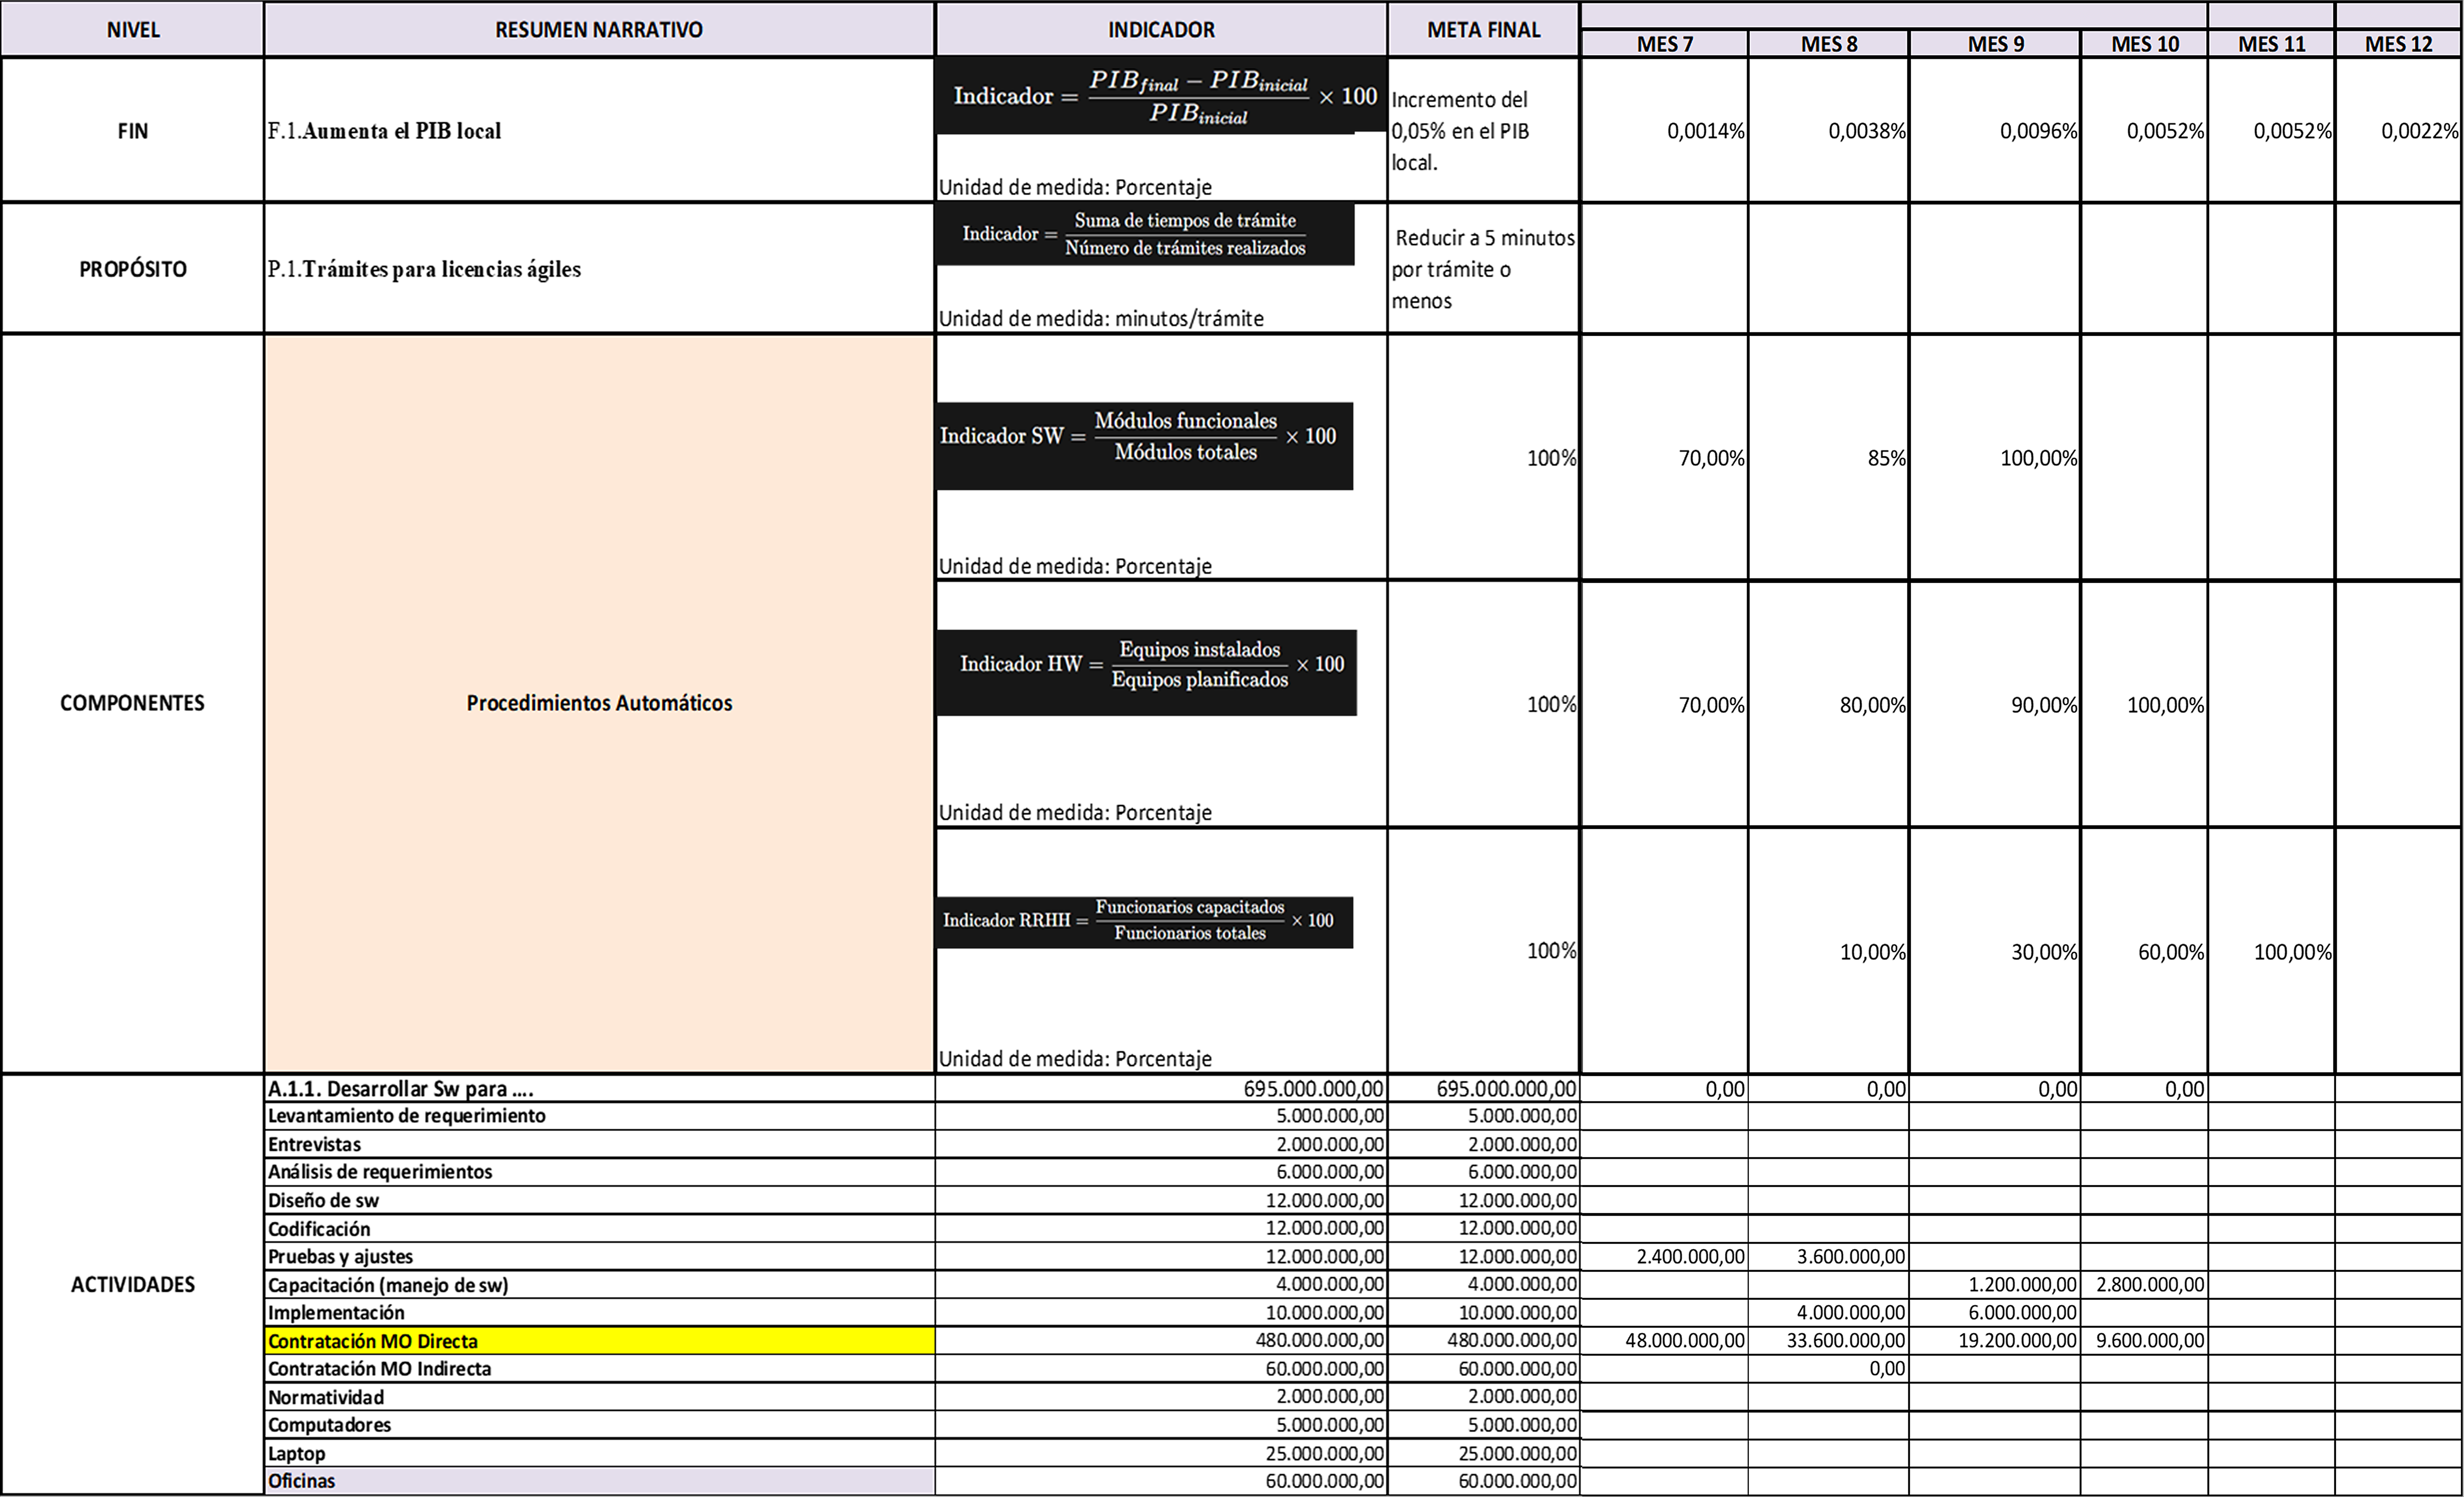
\includegraphics[width=1\linewidth]{indicators/images/indicadores2.png}
    \caption{Matriz de indicadores mes 7 - 12}
     \vspace{0.2cm}
    \small Fuente: Elaboración propia
    \label{tab:indicadores2}
\end{table}%
\end{landscape}

La implementación del sistema propuesto para la Secretaría de Tránsito de Pereira busca optimizar los procesos de expedición de licencias de conducción mediante la automatización de trámites. Este tipo de soluciones busca mejorar el crecimiento del Producto Interno Bruto (PIB) local, gracias a la reducción de costos operativos, el aumento de la productividad del personal y la disminución de tiempos de atención a los ciudadanos.

Diversos estudios internacionales respaldan la relación entre la digitalización del sector público y el crecimiento económico. De acuerdo con el Banco Interamericano de Desarrollo (BID, 2022), los proyectos de modernización digital en gobiernos locales de América Latina han generado aumentos en la productividad de entre 0,5\% y 0,8\% del PIB en un periodo de dos años. Por su parte, un estudio de \textit{McKinsey Global Institute} (McLKinsey, 2011) estimó que la digitalización de servicios públicos puede contribuir con hasta un 1,5\% anual al PIB de las economías en desarrollo. De manera similar, la \textit{OCDE} (OCDE, 2020) indicó que los procesos de transformación digital en instituciones gubernamentales generan incrementos sostenidos en la eficiencia económica entre 0,3\% y 1,0\% anual.

En el contexto colombiano, el DANE reportó que el PIB de Pereira alcanzó aproximadamente 28 billones de pesos en 2023 (DANE, 2024). Considerando esta base y los rangos de crecimiento derivados de la literatura mencionada, se estima que la implementación del sistema digital podría generar un impacto positivo progresivo sobre el PIB local equivalente a un aumento del 0,2\% durante el primer año y de 0,4\% en el segundo año.


\section{Matriz de supuestos}

\begin{figure}[H]
    \centering
    \includegraphics[width=1\linewidth]{mml/images/supuestos.png}
    \caption{Matriz de supuestos}
    \vspace{0.2cm}
    \small Fuente: Elaboración propia
    \label{fig:supuestos}
\end{figure}

\section{Matriz de medios de verificación}

\begin{figure}[H]
    \centering
    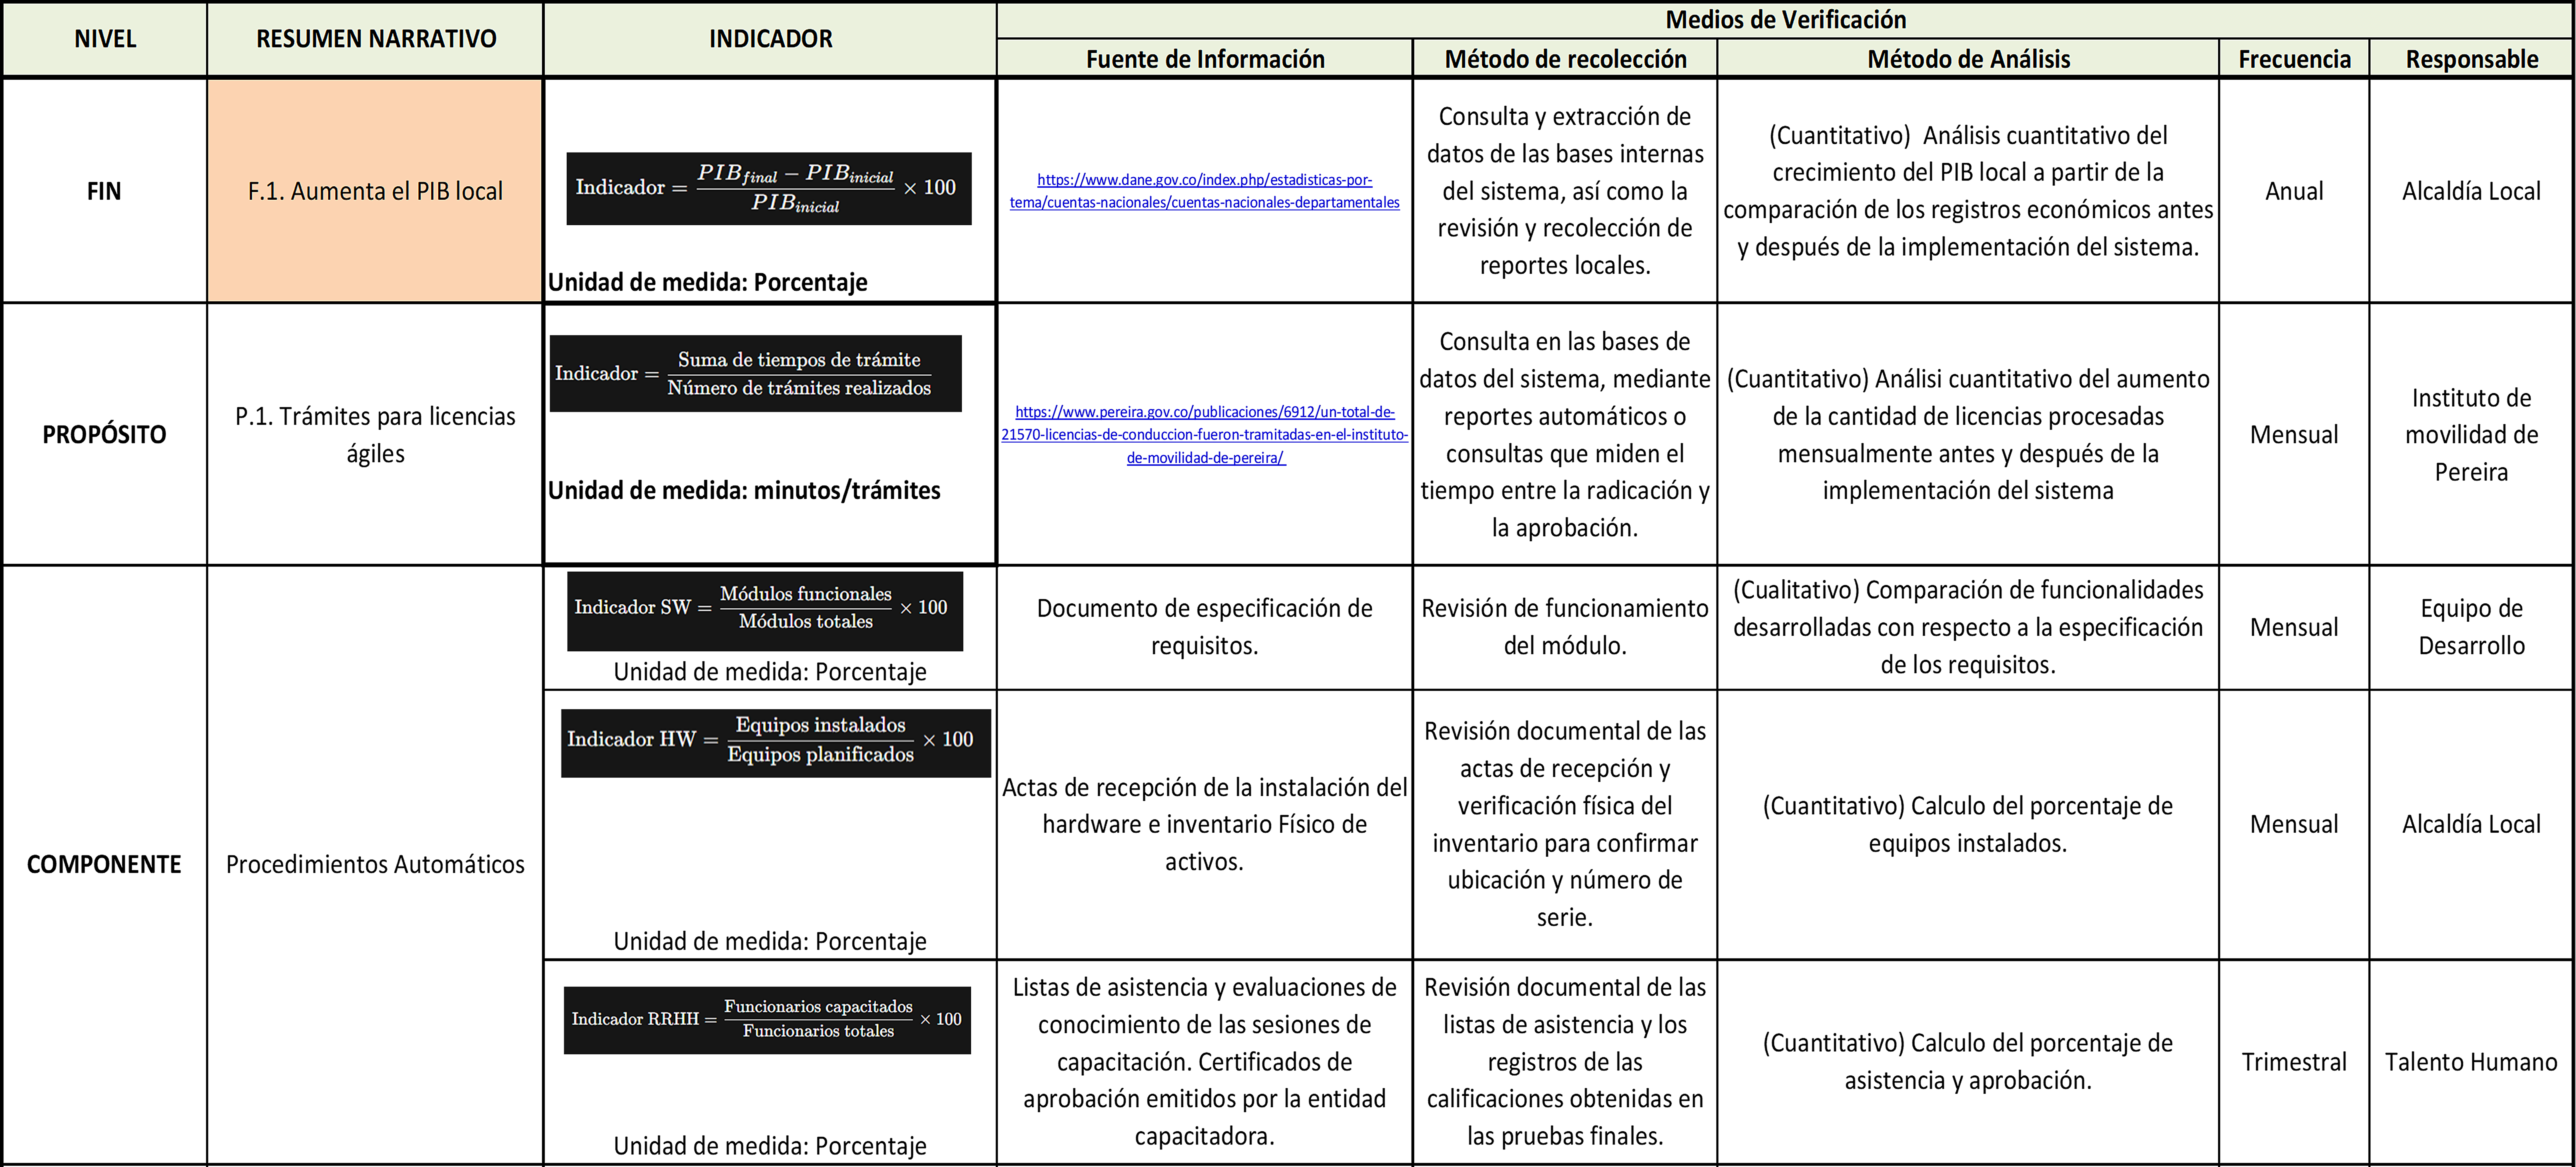
\includegraphics[width=1\linewidth]{mml/images/verificacion1.png}
    \caption{Matriz de medios de verificación - parte 1}
    \vspace{0.2cm}
    \small Fuente: Elaboración propia
    \label{fig:medios de verificación1}
\end{figure}


\begin{figure}[H]
    \centering
    \includegraphics[width=1\linewidth]{mml/images/verificacion2.png}
    \caption{Matriz de medios de verificación - parte 2}
    \vspace{0.2cm}
    \small Fuente: Elaboración propia
    \label{fig:medios de verificación2}
\end{figure}

\section{Matriz de Marco Lógico}

\begin{figure}[H]
    \centering
    \includegraphics[width=1\linewidth]{mml/images/mml1.png}
    \caption{Matriz de Marco Lógico - parte 1}
    \vspace{0.2cm}
    \small Fuente: Elaboración propia
    \label{fig:mml1}
\end{figure}


\begin{figure}[H]
    \centering
    \includegraphics[width=1\linewidth]{mml/images/mml2.png}
    \caption{Matriz de Marco Lógico - parte 2}
    \vspace{0.2cm}
    \small Fuente: Elaboración propia
    \label{fig:mml2}
\end{figure}

\end{document}

% =====================
% Referencias
% =====================
\newpage

%===================================
%===================================
\addcontentsline{toc}{section}{Referencias}
\begin{thebibliography}{99}

\bibitem{RUNT2025}
Registro Único Nacional de Tránsito (RUNT). (2025). \textit{Sitio web oficial}. Recuperado de \url{https://www.runt.com.co}. Consultado el 27 de agosto de 2025.

\bibitem{AlcaldiaPereiraTransito2025}
Alcaldía de Pereira — Secretaría de Tránsito. (2025). \textit{Portal de Tránsito}. Recuperado de \url{https://www.pereira.gov.co/transito}. Consultado el 27 de agosto de 2025.

\bibitem{GobernacionRisaralda2025}
Gobernación de Risaralda. (2025). \textit{Sitio web oficial}. Recuperado de \url{https://www.risaralda.gov.co}. Consultado el 27 de agosto de 2025.

\bibitem{AlcaldiaPereira2025}
Alcaldía de Pereira. (2025). \textit{Sitio web oficial}. Recuperado de \url{https://www.pereira.gov.co}. Consultado el 27 de agosto de 2025.

\bibitem{Bogota2021}
Bogotá.gov.co. (2021, febrero 18). \textit{¿Cuál es la diferencia entre una IPS y una EPS?} Bogotá.gov.co. Recuperado de \url{https://bogota.gov.co/mi-ciudad/salud/cual-es-la-diferencia-entre-una-ips-y-una-eps}

\bibitem{CEA-sf}
Centro de Enseñanza Automovilística (CEA). (s/f). \textit{Com.co}. Recuperado de \url{https://movilidadtotal.com.co/centro_de_ensenanza_automovilistica_cea/}

\bibitem{CRC2023}
Centro de Reconocimiento de Conductores CRC. (2023, junio 26). \textit{Proteger IPS}. Recuperado de \url{https://www.protegerips.com/centro-de-reconocimiento-de-conductores-crc/}

\bibitem{Minsalud-sf-a}
Colombia, M. de S. y. P. S. (s/f). \textit{Páginas - Instituciones Prestadoras de Servicios de Salud Acreditadas}. Gov.co. Recuperado de \url{https://www.minsalud.gov.co/salud/CAS/paginas/instituciones-prestadoras-de-salud-ips-acreditadas.aspx}

\bibitem{ElPereirano2023a}
El Pereirano. (2023). \textit{Problemas de movilidad y seguridad afectan a Pereira y Dosquebradas}. Recuperado de \url{https://elpereirano.com/2023/05/06/problemas-de-movilidad-y-seguridad-afectan-a-pereira-y-dosquebradas}

\bibitem{PaseDeMoto2025}
PaseDeMoto. (2025). \textit{Licencia de Conducción Pereira – Requisitos y Trámite}. Recuperado de \url{https://pasedemoto.com/licencias-de-conduccion/pereira}

\bibitem{RCN2023}
RCN Radio. (2023). \textit{En Pereira hacen falta al menos 130 agentes de tránsito}. Recuperado de \url{https://www.rcnradio.com/colombia/eje-cafetero/en-pereira-hacen-falta-al-menos-130-agentes-de-transito}

\bibitem{ElPereirano2023b}
El Pereirano. (2023). \textit{Déficit de 120 agentes de tránsito en Pereira}. Recuperado de \url{https://elpereirano.com/2023/02/24/deficit-de-120-agentes-de-transito-en-pereira}

\bibitem{ConcejoPereira2023}
Concejo de Pereira. (2023). \textit{Más agilidad en la renovación de licencias de conducción piden los concejales de Pereira}. Recuperado de \url{https://www.concejopereira.gov.co/es/mas-agilidad-en-la-renovacion-de-licencias-de-conduccion-piden-los-concejales-de-pereira-EV2305}

\bibitem{RCN2024}
RCN Radio. (2024). \textit{Caídas del RUNT paralizan trámites en Pereira}. Recuperado de \url{https://www.noticiasrcn.com/colombia/caidas-del-runt-paralizan-tramites-en-pereira-2024}

\bibitem{Infobae2024}
Infobae. (2024). \textit{Pico y placa solidario, cursos pedagógicos y trámites en ventanilla única no podrán realizarse este lunes por cierre de la plataforma RUNT}. Recuperado de \url{https://www.infobae.com/colombia/2024/06/24/pico-y-placa-solidario-cursos-pedagogicos-y-tramites-en-ventanilla-unica-no-podran-realizarse-este-lunes-por-cierre-de-la-plataforma-runt}

\bibitem{LaRepublica2025}
La República. (2025). \textit{Una empresa en Colombia debe destinar 2.620 horas al año en trámites administrativos}. Recuperado de \url{https://www.larepublica.co/economia/una-empresa-en-colombia-debe-destinar-2-620-horas-al-ano-en-tramites-administrativos-4210833}

\bibitem{ValoraAnalitik2025}
Valora Analitik. (2025). \textit{Los dos megaproyectos clave para Bogotá que aún no arrancan por trámites administrativos}. Recuperado de \url{https://www.valoraanalitik.com/primicia-los-dos-megaproyectos-clave-para-bogota-que-se-adjudicaron-en-2022-y-no-han-arrancado-estas-son-las-razones}

\bibitem{Corficolombiana2025}
Corficolombiana. (2025). \textit{Informe sobre impacto económico de la tramitología en Colombia}.

\bibitem{Aditt-sf}
Aditt.org. (s/f). \textit{Conózcanos}. Recuperado de \url{https://aditt.org/conozcanos/}

\bibitem{Corte-sf}
Corte Constitucional. (s. f.). \textit{Definición de EPS e IPS}. Relatoría Constitucional. Recuperado de \url{https://www.corteconstitucional.gov.co/}

\bibitem{FND-sf}
Federación Nacional de Departamentos. (s. f.). \textit{Risaralda}. Federación Nacional de Departamentos. Recuperado de \url{https://fnd.org.co/departamentos/risaralda}

\bibitem{FOPEP-sf}
Fondo de Pensiones de Colombia (FOPEP). (s. f.). \textit{Entidad bancaria}. FOPEP. Recuperado de \url{https://www.fopep.gov.co/glosario/entidad-bancaria}

\bibitem{GrupoR5-sf}
Grupo R5. (s. f.). \textit{¿Qué es el RUNT y para qué sirve?} Grupo R5. Recuperado de \url{https://www.grupor5.com/aprende/vehiculos/que-es-el-runt}

\bibitem{HospitalNecocli-sf}
Hospital Necoclí. (s. f.). \textit{Entidades del sector salud}. Hospital de Necoclí. Recuperado de \url{https://www.hospitalnecocli.gov.co/}

\bibitem{Informacolombia-sf}
Informacolombia. (s. f.). \textit{Asociación Taxistas Risaralda}. Informacolombia. Recuperado de \url{https://www.informacolombia.com/directorio-empresas/informacion-empresa/asociacion-taxistas-risaralda}

\bibitem{INS-sf}
Instituto Nacional de Salud. (s. f.). \textit{Objeto y funciones}. Instituto Nacional de Salud. Recuperado de \url{https://www.ins.gov.co/}

\bibitem{Inter-sf}
Inter Rapidísimo. (s. f.). \textit{Servicio de mensajería exprés}. Inter Rapidísimo. Recuperado de \url{https://interrapidisimo.com/servicio-mensajeria-expresa}

\bibitem{Ley100-1993}
Congreso de la República de Colombia. (1993). \textit{Ley 100 de 1993. Sistema General de Seguridad Social en Salud}.

\bibitem{MinTransporte2025}
Ministerio de Transporte. (2025, abril). \textit{MinTransporte anunció cierre del RUNT este 23 de abril; ¿qué pasará con la plataforma?} Tropicana FM. Recuperado de \url{https://www.tropicanafm.com/2025/mintransporte-anuncio-cierre-del-runt-este-23-de-abril-que-pasara-con-la-plataforma-433700.html}

\bibitem{Minsalud-sf-b}
Ministerio de Salud y Protección Social. (s. f.). \textit{Institucional}. Ministerio de Salud y Protección Social. Recuperado de \url{https://www.minsalud.gov.co/}

\bibitem{Mintransporte2011}
Mintransporte. (2011, mayo 8). \textit{¿Quiénes somos?} Mintransporte. Recuperado de \url{https://mintransporte.gov.co/publicaciones/33/quienes-somos/}

\bibitem{AMCO2020}
Occidente, Á. M. C. (2020, mayo 4). \textit{¿Quiénes somos?} Área Metropolitana Centro de Occidente. Recuperado de \url{https://www.amco.gov.co/publicaciones/102/quienes-somos/}

\bibitem{RUNT-sf-a}
Gov.co. (s/f). \textit{¿Qué es el RUNT?} Recuperado de \url{https://www.runt.gov.co/sobre-runt/que-es-runt}

\bibitem{Pereira2023}
Pereira, S. E. (2023, 13 febrero). \textit{Instituto Municipal de Movilidad de Pereira}. Sede Electrónica de Pereira. Recuperado de \url{https://www.pereira.gov.co/espectaculo-publico/publicaciones/6322/instituto-municipal-de-movilidad-de-pereira/}

\bibitem{SigoSeguros2024}
Sigo Seguros. (2024, diciembre 6). \textit{¿Qué es una agencia de seguros y cómo funciona?} Sigo Seguros. Recuperado de \url{https://sigoseguros.com/blog/que-es-una-agencia-de-seguros-y-como-funciona}

\bibitem{TusDatos2025}
TusDatos. (2025, mayo 22). \textit{¿Qué es el RUNT y qué información te brinda?} TusDatos.co. Recuperado de \url{https://www.tusdatos.co/blog/que-es-el-runt-y-que-informacion-te-brinda}

\bibitem{Wikipedia-sf}
Wikipedia. (s. f.). \textit{Autoescuela}. En Wikipedia. Recuperado de \url{https://es.wikipedia.org/wiki/Autoescuela}

\bibitem{AGN2024}
Archivo General de la Nación. (2024). \textit{Acuerdo 001 de 2024. Por el cual se establece el Acuerdo Único de la Función Archivística, se definen los criterios técnicos y jurídicos para su implementación en el Estado Colombiano y se fijan otras disposiciones}. \url{https://sedeelectronica.sic.gov.co/sites/default/files/normativa/POLITICA%20DE%20DOCUMENTOS%20ELECTRONICOS%20DE%20ARCHIVO.pdf}

\bibitem{AGNMinTIC2020}
Archivo General de la Nación \& Ministerio de Tecnologías de la Información y las Comunicaciones. (2020). \textit{Protocolo para Digitalización de Documentos con Fines Probatorios}. \url{https://www.unidadvictimas.gov.co/wp-content/uploads/2020/07/5.Programa_de_Reprografia_Y_Digitalizacion_Con_Fines_Probatorios_V3.pdf}

\bibitem{Ley527}
Congreso de la República de Colombia. (1999). \textit{Ley 527 de 1999. Por medio de la cual se define y reglamenta el acceso y uso de los mensajes de datos, del comercio electrónico y de las firmas digitales, y se dictan otras disposiciones}. \url{https://www.funcionpublica.gov.co/eva/gestornormativo/norma.php?i=4276}

\bibitem{Ley594}
Congreso de la República de Colombia. (2000). \textit{Ley 594 de 2000. Por medio de la cual se dicta la Ley General de Archivos y se dictan otras disposiciones}. \url{https://www.funcionpublica.gov.co/eva/gestornormativo/norma.php?i=4275}

\bibitem{Ley769}
Congreso de la República de Colombia. (2002). \textit{Ley 769 de 2002. Por la cual se expide el Código Nacional de Tránsito Terrestre y se dictan otras disposiciones}. \url{https://www.oas.org/juridico/spanish/mesicic2_col_ley_769_2002.pdf}

\bibitem{Ley1581}
Congreso de la República de Colombia. (2012). \textit{Ley 1581 de 2012. Por la cual se dictan disposiciones generales para la protección de datos personales}. \url{https://www.funcionpublica.gov.co/eva/gestornormativo/norma.php?i=49981}

\bibitem{ISO27001}
International Organization for Standardization/International Electrotechnical Commission. (2022). \textit{ISO/IEC 27001:2022: Sistemas de gestión de la seguridad de la información}. \url{https://www.mintic.gov.co/portal/715/articles-403045_recurso_1.pdf}

\bibitem{MinTICEstandares}
Ministerio de Tecnologías de la Información y las Comunicaciones. (s.f.). \textit{Estándares y Tecnologías}. \url{https://www.mintic.gov.co/portal/inicio/5236:Estandares-y-Tecnologias}

\bibitem{MinTICNube}
Ministerio de Tecnologías de la Información y las Comunicaciones. (s.f.). \textit{Lineamientos de seguridad de la información para el uso de servicios en la nube}. \url{https://gobiernodigital.mintic.gov.co/692/articles-401777_recurso_1.pdf}

\bibitem{MinTICSeguridadDigital}
Ministerio de Tecnologías de la Información y las Comunicaciones. (s.f.). \textit{Política de Seguridad Digital. [Preguntas Frecuentes]}. \url{https://www.mintic.gov.co/portal/inicio/Atencion-y-Servicio-a-la-Ciudadania/Preguntas-frecuentes/15430:Politica-de-Seguridad-Digital}

\bibitem{MinTICPlanSeguridad}
Ministerio de Tecnologías de la Información y las Comunicaciones. (2025). \textit{Plan de seguridad y privacidad de la información}. \url{https://www.mintic.gov.co/portal/inicio/Planes/Plan-de-seguridad-y-privacidad-de-la-informacion/}

\bibitem{Resolucion0312}
Ministerio del Trabajo. (2019). \textit{Resolución 0312 de 2019. Por la cual se definen los Estándares Mínimos del Sistema de Gestión de la Seguridad y Salud en el Trabajo SG-SST}. \url{https://metd.com.co/resolucion-0312-2019-estandares-minimos-sg-sst/}

\bibitem{Resolucion12336}
Ministerio de Transporte. (2012). \textit{Resolución 12336 de 2012. Por la cual se establecen los parámetros técnicos para la evaluación de las condiciones físicas, mentales y de coordinación motriz para obtener o renovar la licencia de conducción}. \url{https://www.runt.gov.co/sites/default/files/normas/resoluciones_12336_del_2012.pdf}

\bibitem{Resolucion9425}
Ministerio de Transporte. (2022, 24 de febrero). \textit{Resolución 0009425 de 2022. Por la cual se modifica y adiciona la Resolución 3245 de 2009}. \url{https://www.runt.gov.co/sites/default/files/normas/MinTransporte-Resolucion-2022-N0009425_20220224.pdf}

\bibitem{DirectivaPresidencial02}
Presidencia de la República de Colombia. (2022, 24 de febrero). \textit{Directiva Presidencial 02 de 2022}. \url{https://www.alcaldiabogota.gov.co/sisjur/normas/Norma1.jsp?i=187174}

\bibitem{Decreto767}
Presidencia de la República de Colombia. (2022). \textit{Decreto 767 de 2022. Por el cual se establecen los lineamientos generales de la Política de Gobierno Digital}. \url{https://www.fondoadaptacion.gov.co/images/2024/Poliitica_Gobierno_Digital/Politica_de_Gobierno_Digital.pdf}

\bibitem{CircularSIC2024}
Superintendencia de Industria y Comercio. (2024). \textit{Circular 1 de 2024. Modificación a la Circular Única en el Título V sobre Datos Personales}. \url{https://normograma.mintic.gov.co/mintic/compilacion/docs/circular_superindustria_0001_2024.htm}

\bibitem{Resolucion5782}
Superintendencia de Puertos y Transporte. (2013). \textit{Resolución 5782 de 2013. Por la cual se establece fecha para hacer exigible a los Centros de Reconocimiento de Conductores -CRC- el sistema de Control y Vigilancia}. \url{https://www.supertransporte.gov.co/documentos/2013/notificaciones/resoluciones_generales/5782.pdf}

\bibitem{ExternadoBiometria}
Universidad Externado de Colombia. (2024, 4 de septiembre). \textit{La SIC actúa contra empresa de criptomonedas por recolección de datos biométricos}. [Artículo de prensa]. \url{https://www.uexternado.edu.co/proteccion-de-datos/la-sic-actua-contra-empresa-de-criptomonedas-por-recoleccion-de-datos-biometricos/}

\bibitem{macbookair}
\textit{Computador Portátil MacBook Air}. \url{https://co.tiendasishop.com/collections/macbook-air}. Consultado: 2025-10-08.

\bibitem{sillaergonomica}
\textit{Silla Ergonómica - Búsqueda en Mercado Libre Colombia}. \url{https://listado.mercadolibre.com.co/silla-ergonomica}. Consultado: 2025-10-08.

\bibitem{escritorioikea}
\textit{Escritorios y escritorios para ordenador - IKEA Colombia}. \url{https://www.ikea.com/co/es/cat/escritorios-20649/}. Consultado: 2025-10-08.

\bibitem{arriendooficina}
\textit{Oficinas en Arriendo en Pereira - Ciencuadras}. \url{https://www.ciencuadras.com/arriendo/pereira/oficina}. Consultado: 2025-10-08.

\bibitem{impresoracarnets}
\textit{Impresora De Carnets A Una Cara Zebra Zc100 Usb}. \url{https://www.mercadolibre.com.co/impresora-de-carnets-a-una-cara-zebra-zc100-usb/up/MCOU2405660816}. Consultado: 2025-10-08.

\bibitem{ribbonimpresora}
\textit{Ribbon para Impresora de Carnets PVC - Búsqueda en Mercado Libre}. \url{https://listado.mercadolibre.com.co/impresora-carnets-pvc}. Consultado: 2025-10-08.

\bibitem{lectorbiometrico}
\textit{Lector Biometrico Usb Digital Persona Uareu 4500}. \url{https://www.mercadolibre.com.co/lector-biometrico-usb-digital-persona-uareu-4500/p/MCO27809732}. Consultado: 2025-10-08.

\bibitem{escanerdocumentos}
\textit{Escáner Portátil de Documentos Workforce ES-50}. \url{https://frontier.com.co/escaner-portatil-de-documentos-workforce-es-50}. Consultado: 2025-10-08.

\bibitem{hostingaws}
\textit{Precios de los servicios en la nube de AWS}. \url{https://aws.amazon.com/pricing/}. Consultado: 2025-10-08.

\bibitem{pasarelapago}
\textit{Top Ten Payment Gateways For Colombian Businesses}. \url{https://muralpay.com/blog/top-ten-payment-gateways-for-colombian-businesses}. Consultado: 2025-10-08.

\bibitem{salariodev}
\textit{Sueldos para Desarrollador de software en Colombia - Indeed}. \url{https://co.indeed.com/career/desarrollador-de-software/salaries}. Consultado: 2025-10-08.

\bibitem{salariopm}
\textit{Empleos de Project manager en Pereira - Indeed}. \url{https://co.indeed.com/jobs?q=project+manager}. Consultado: 2025-10-08.

\bibitem{salariotester}
\textit{Empleos de QA Tester - Indeed}. \url{https://co.indeed.com/viewjob?jk=88ffff663daf3ab3}. Consultado: 2025-10-08.

\bibitem{lapicerosbic}
\textit{Plumas Lapicero Bic Dura+ Punto Mediano 1 Mm Caja 50}. \url{https://www.mercadolibre.com.co/plumas-lapicero-bic-dura-punto-mediano-1-mm-caja-50-th/p/MCO2038834926}. Consultado: 2025-10-08.

\bibitem{soportesalescloud}
\textit{Soporte Técnico Informático para Empresas - Sales Cloud}. \url{https://salescloud.com.co/soporte-tecnico/modalidad-tarifas/}. Consultado: 2025-10-08.

\bibitem{cafequindio}
\textit{Tripack Café Gourmet - Café Quindío}. \url{https://www.cafequindio.com.co/products/tripack-cafe-gouermet}. Consultado: 2025-10-08.

\bibitem{capacitacionunir}
Aguiar Ulloa, D. V. (s.f.). \textit{Elaboración de un plan de capacitación por competencias para los servidores públicos}. \url{https://reunir.unir.net/bitstream/handle/123456789/5594/AGUIAR%20ULLOA%2C%20DOUGLAS.pdf?isAllowed=y&sequence=1}. Consultado: 2025-10-08.

\bibitem{DANE2024}
Departamento Administrativo Nacional de Estadística (DANE). (2024). \textit{Proyecciones y retroproyecciones de población municipal, 2018--2042}. Recuperado de \url{https://www.dane.gov.co/index.php/estadisticas-por-tema/demografia-y-poblacion/proyecciones-de-poblacion}

\bibitem{IMP2024}
Instituto de Movilidad de Pereira. (2024). \textit{Informe de gestión — Corte 30 de noviembre de 2024}. Pereira: Instituto de Movilidad de Pereira. Recuperado de \url{https://movilidadpereira.gov.co/Documentos/Dependencias/2024/planeacion/INFORMEDEGESTION30DENOVIEMBREDE2024.pdf}

\bibitem{AGN2024}
Archivo General de la Nación. (2024). \textit{Acuerdo 001 de 2024. Por el cual se establece el Acuerdo Único de la Función Archivística, se definen los criterios técnicos y jurídicos para su implementación en el Estado Colombiano y se fijan otras disposiciones}. Recuperado de \url{https://sedeelectronica.sic.gov.co/sites/default/files/normativa/POLITICA%20DE%20DOCUMENTOS%20ELECTRONICOS%20DE%20ARCHIVO.pdf}

\bibitem{BID2022}
Banco Interamericano de Desarrollo. (2022). \textit{El auge de GovTech en América Latina y el Caribe: hacia un sector público más ágil, eficiente y transparente}. Washington, D.C. Recuperado de \url{https://publications.iadb.org/es/el-auge-de-govtech-en-america-latina-y-el-caribe}

\bibitem{McKinsey2011}
McKinsey Global Institute. (2011). \textit{Internet matters: The Net’s sweeping impact on growth, jobs, and prosperity}. McKinsey \& Company. Recuperado de \url{https://www.mckinsey.com/industries/technology-media-and-telecommunications/our-insights/internet-matters}

\bibitem{OCDE2020}
Organización para la Cooperación y el Desarrollo Económicos (OCDE). (2020). \textit{Digital Government Index: 2019 Results}. OECD Public Governance Policy Papers, No. 03. París: OECD Publishing. \url{https://doi.org/10.1787/4de9f5bb-en}

\bibitem{DANE2024}
Departamento Administrativo Nacional de Estadística (DANE). (2024). \textit{Cuentas nacionales departamentales: Producto Interno Bruto por departamento 2023}. Bogotá D.C. Recuperado de \url{https://www.dane.gov.co/index.php/estadisticas-por-tema/cuentas-nacionales/cuentas-nacionales-departamentales}


\end{thebibliography}


\end{document}